% !TeX root = ../main.tex

\chapter{详细设计与实现}

本章将在第4章的基础上对划分出来的各个模块进行更为详细的设计与实现。一方面通过类图的形式,展现在本模块中各个类之间的关系,通过类的属性和接口设计,相互配合完成本模块的功能;另一方面,对于比较复杂重要的方法实现,采用流程图的形式,详细介绍其内部的实现逻辑和流程。

\section{图信息保存模块设计与实现}

图信息保存模块是整个编译优化中避免重复编译的基础,只有在能保存下用户图信息的基础上,才能继续实现图信息识别和指令替换等功能。图信息保存模块要实现将操作的结构和数据信息保存到对应的Json对象,最后将Json像的内容转输出成可读的Json文件,该模块类图设计如图~\ref{fig:info-save-model}所示。

\begin{figure}[htb]
  \centering
  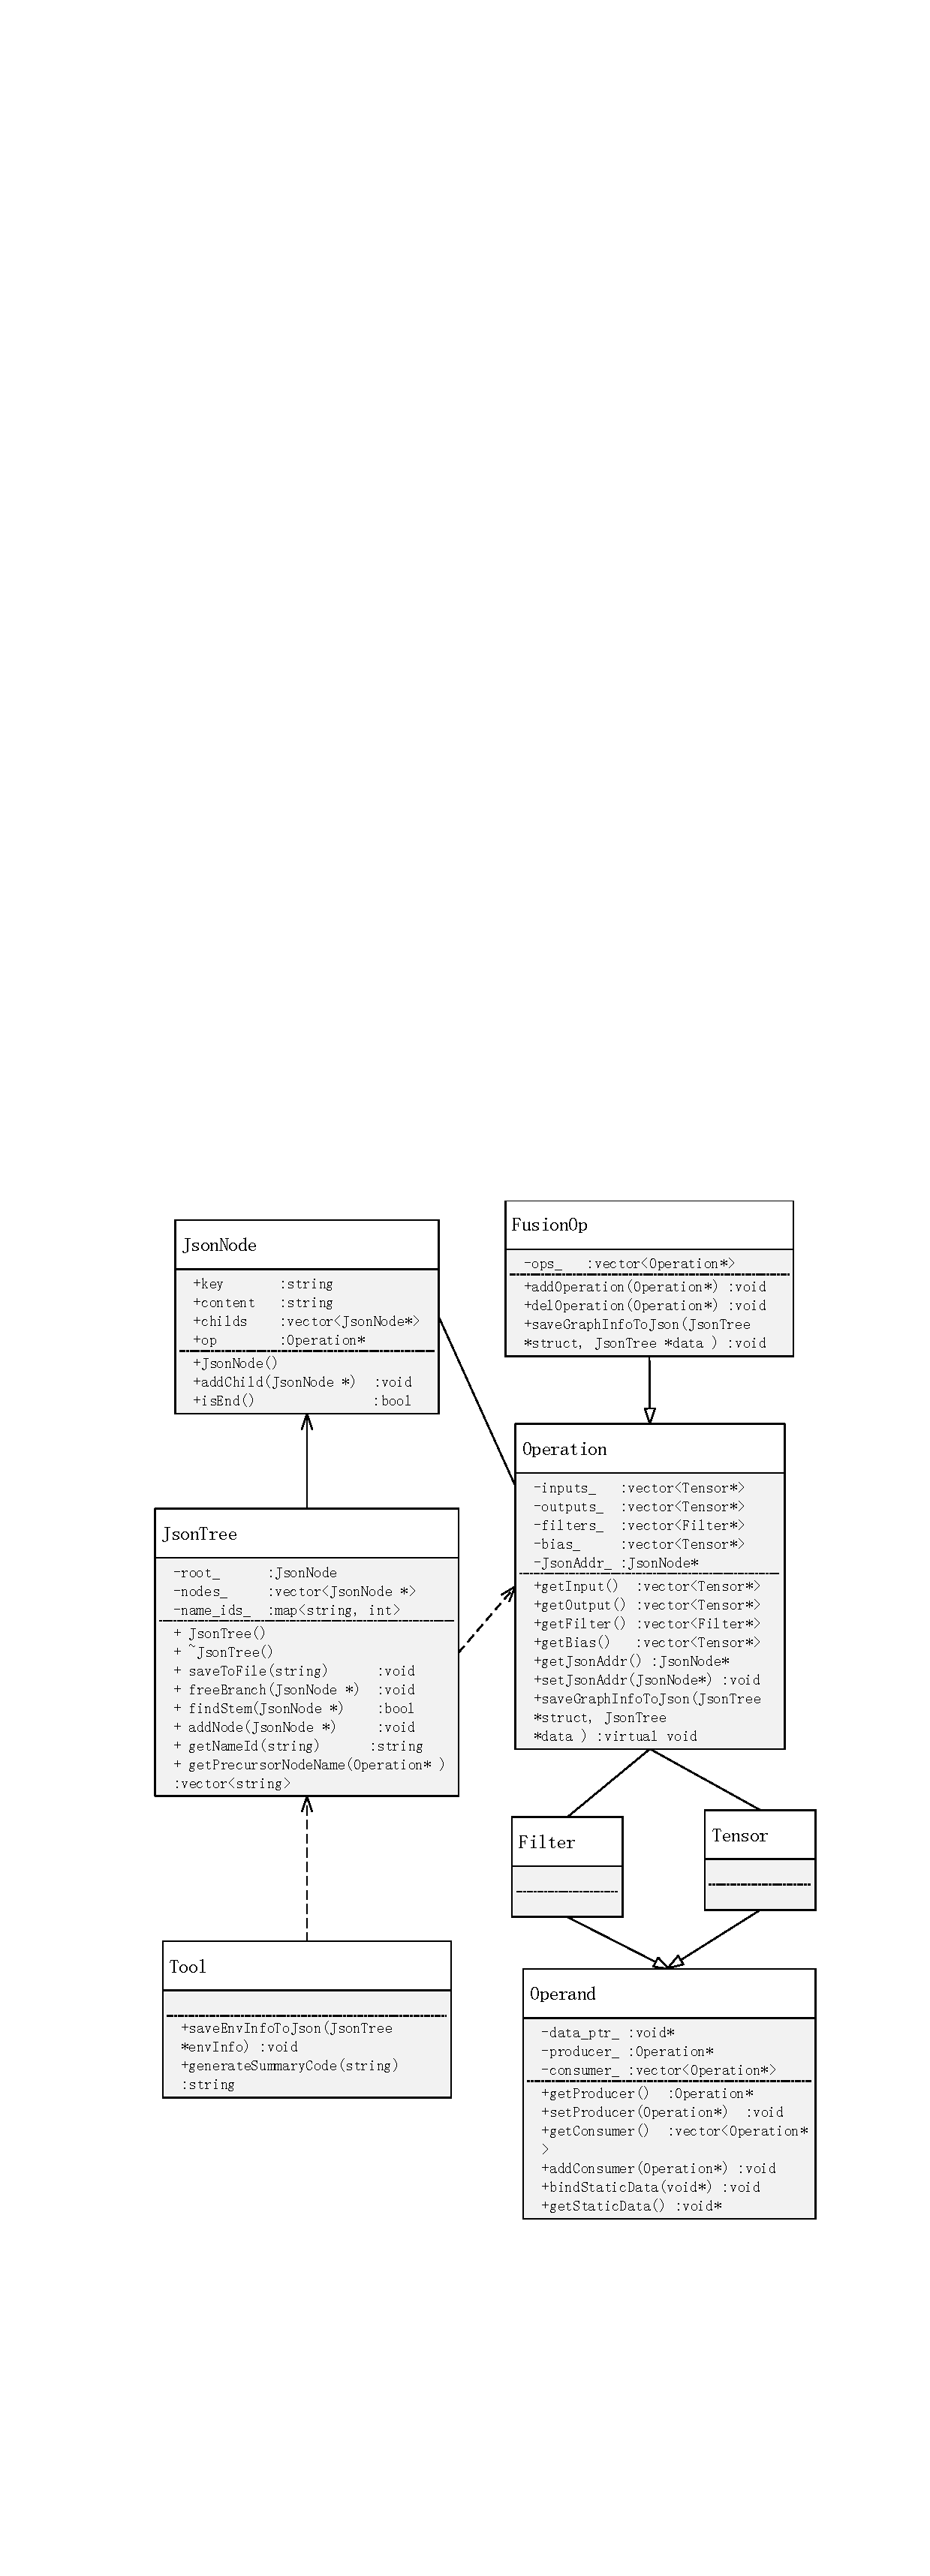
\includegraphics[width=0.6\textwidth]{info_save_model.pdf}
  \caption{图信息保存模块类图}
  \label{fig:info-save-model}
\end{figure}

各个类主要函数的功能在表~\ref{tab:function-list}中做了简要说明。
\begin{table}[htb]
  \centering\tiny
  \caption{函数功能表}
  \label{tab:function-list}
  \begin{tabular}{llll}
    \toprule
    类名        & 函数名     & 功能      & 说明                \\
    \midrule
    JsonNode   & addChild  & 添加子节点     & 仅仅当content为空时才有效 \\
               & isEnd     & 判断是否是终点 & 保存到文件中是用来判读是否是结尾\\
    \midrule
    JsonTree   & saveToFile  & 将JsonTree的内容保存到文件中  &  \\
               & freeBranch  & 释放指定分支 & 析构时使用\\
               & saveStemToFile & 保存指定分支到文件中 & \\
               & addNode & 添加子节点 & \\
               & getNameId & 查找同类型的节点的数量& 输入操作的名称,字典name\_id\_对应该名称对应的个数 \\
               & getPrecursorNodeName & 查找指定操作所有前驱节点的name & 通过操作和Tensor来判断前驱和后继的关系\\ 
    \midrule
    FusionOp   & addOperation  & 向计算图中添加子操作    &  \\
               & delOperation  & 删除计算图中指定的操作 &  \\ 
               & saveGraphInfoToJson & 保存计算图的结构和数据信息 & 通过调用其中的子操作实现 \\
    \midrule
    Operation  & getInput   & 获取输入Tensor    &  \\
               & getOutput  & 获取输出Tensor &  \\ 
               & getFilter  & 获取filter & \\
               & getBias    & 获取bias  & \\
               & getJsonAddr& 获取操作对应JsonNode的指针 & \\
               & saveGraphInfoToJson & 保存结构信息到对应的JsonTree中 & 虚函数,子类根据自身实际情况实现 \\
               & saveDataInfoToJson & 保存静态数据信息到JsonTree中 & 在基类中实现 \\
    \midrule
    Tool       & saveEnvInfoToJson   & 保存环境信息到JsonTree中  \\
               & generateSummaryCode & 根据输入内容生成信息摘要编码  &使用MD5码算法实现,返回长16个字符的编码\\
    \midrule
    Operand    & getProducer  & 找操作数的生产者  &每个操作数只有一个生产者,即它只能是/一个操作的输出 \\
               & getConsumer  & 找操纵数的消费者  &每个操作可能有多个消费者,即它可以是多个操作的输入 \\
               & bindStaticData  & 绑定静态数据信息  & 静态数据信息的绑定应该在编译之前完成\\
               & getStaticData   & 获取静态数据地址  & \\ 
    \bottomrule 
  \end{tabular}
\end{table}

在~\ref{fig:info-save-model}的类图中可以看出,图信息实际上都是保存在JsonTree的实例化对像中。因为环境信息不依赖与任何操作而只与当前的运行环境相关,所以直接方法工具类Tool中实现,结构信息和权值信息都和操作相关,所以放到操作中实现。工具类Tool中还实现了另一个重要的方法generateSummaryCode,用于生成字符串对应的信息摘要编码。操作中保存图信息的入口是基类Operation中的虚函数saveGraphInfoToJson,子类操作实现该接口将自己的信息加入到JsonTree中。包含有多个操作的图用FusionOp表示,FusionOp的图信息保存通过遍历调用包含在其中的子操作对应的接口实现。

信息存在JsonTree中,而JsonTree实际上是由一个个的JsonNode组成,JsonNode可以有多种方式存放信息。如果是string-string类型的键值对,则可以直接用key和content保存内容;如果键值对中值的类型是一个或多个Json对象,则可以保存到childNodes中。这样就可以通过增加子节点的方式,逐级拓展下去。


\subsection {保存结构信息}
接下来详细介绍操作的saveGraphInfoToJson函数如何利用各种接口实现将计算图的结构信息存储到JsonTree中的,saveGraphInfoToJson实现步骤如流程图~\ref{fig:save-graph-info}所示。

\begin{figure}[htb]
  \centering
  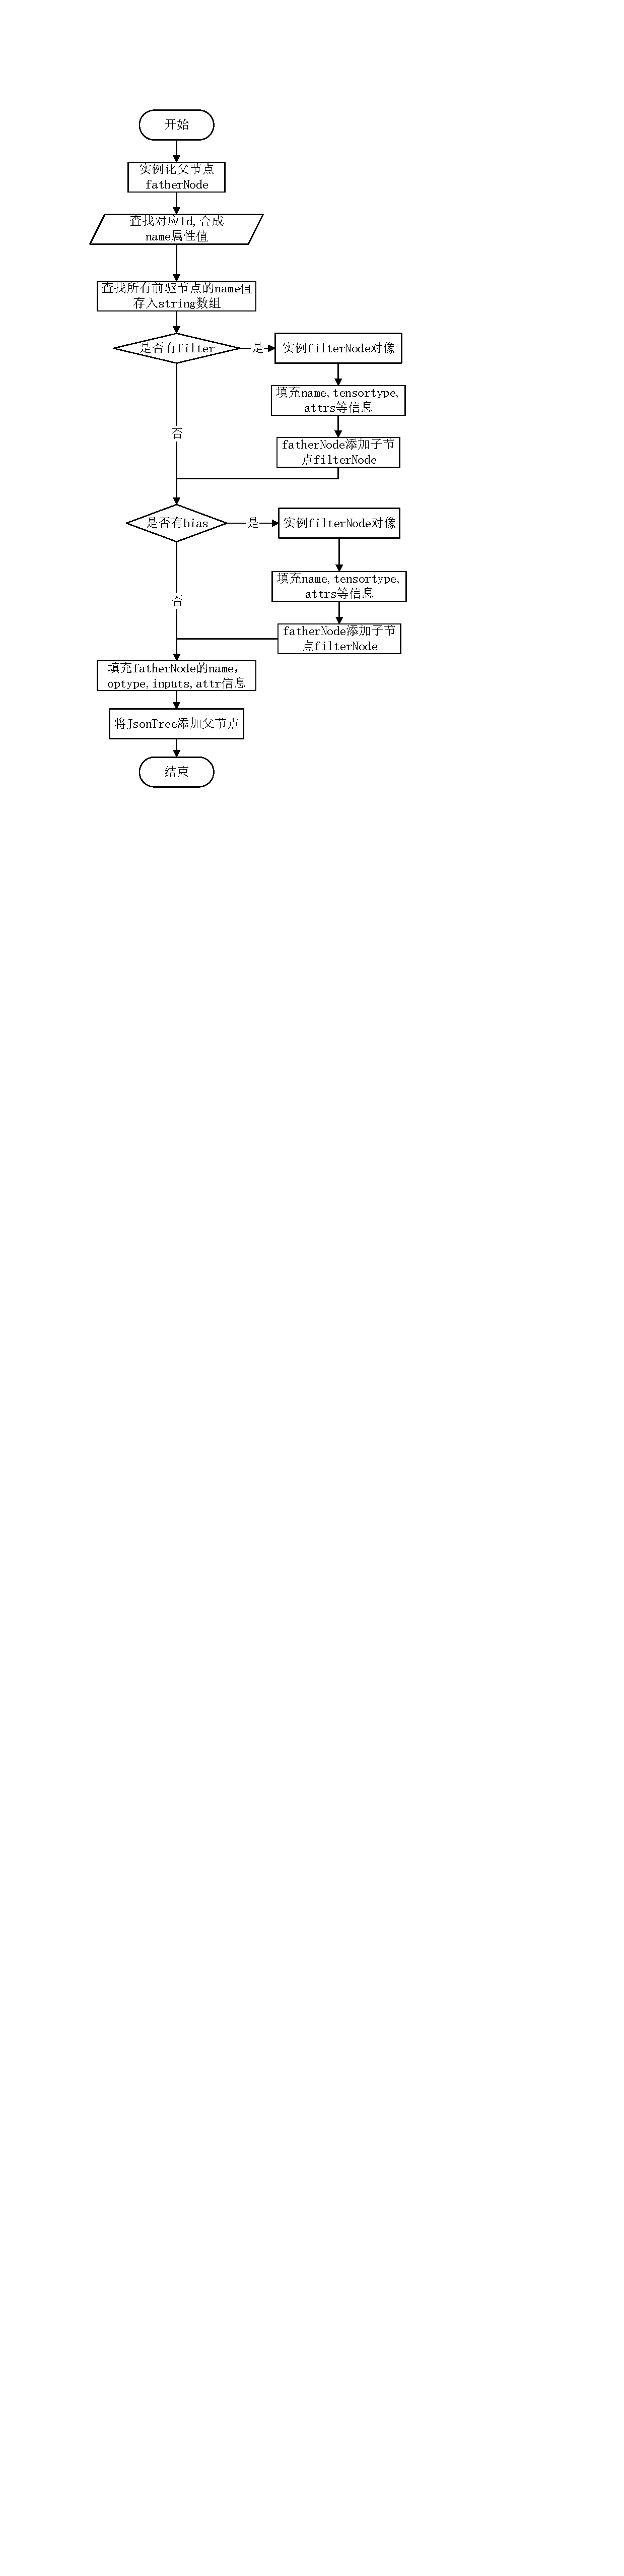
\includegraphics[width=0.4\textwidth]{save_graph_info.pdf}
  \caption{saveGraphInfoToJson流程图}
  \label{fig:save-graph-info}
\end{figure}

在图~\ref{fig:save-graph-info}中,每个操作都要实例化和直接对应一个JsonNode,实例化之后,Operation中的jsonAddr\_指向这个实例化的对象,同时JsonNode中的op指针也指向当前操作。唯一标识符name由类型名和Id号两部分组成,当JsonTree中出现多个conv类型节点时会以conv1,conv2…的形式命名,所以要查找当前Id来合成name。接下来较为麻烦的一步是需要查找出当前节点的输入来自于哪些节点,需要将这些节点的name信息写入到inputs中。然后根据操作输入是否存在filter和bias来决定是否需要添加filter和bias的信息,并将filter和bias的name值也写入到当前节点的inputs中。最后补充name,optype,attrs字段的信息,并将操作节点添加到JsonTree。

查找前驱节点是通过JsonTree的getPrecursorNodeName函数来实现,其逻辑如图~\ref{fig:get-precursor-node}所示。

\begin{figure}[htb]
  \centering
  \subfigure[getPrecursorNodeName流程图]{
  \label{fig:get-precursor-node}
  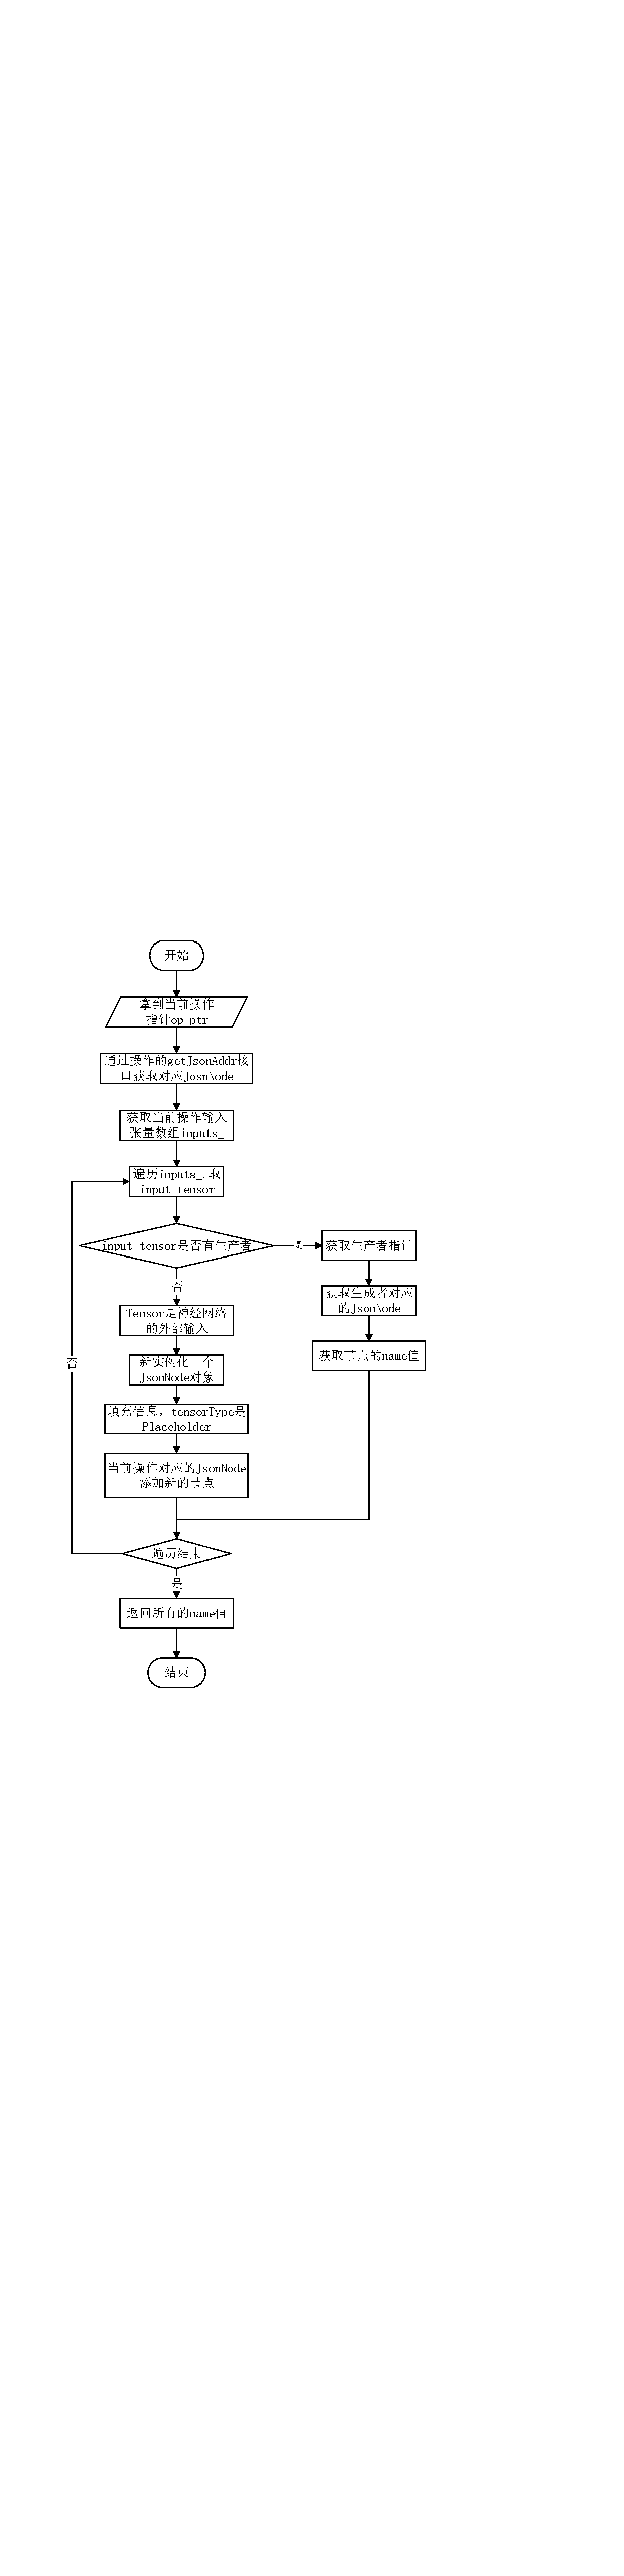
\includegraphics[width=0.4\textwidth]{get_precursor_node.pdf}
  }
  \subfigure[保存权值流程图]{
  \label{fig:save-weight-info}
  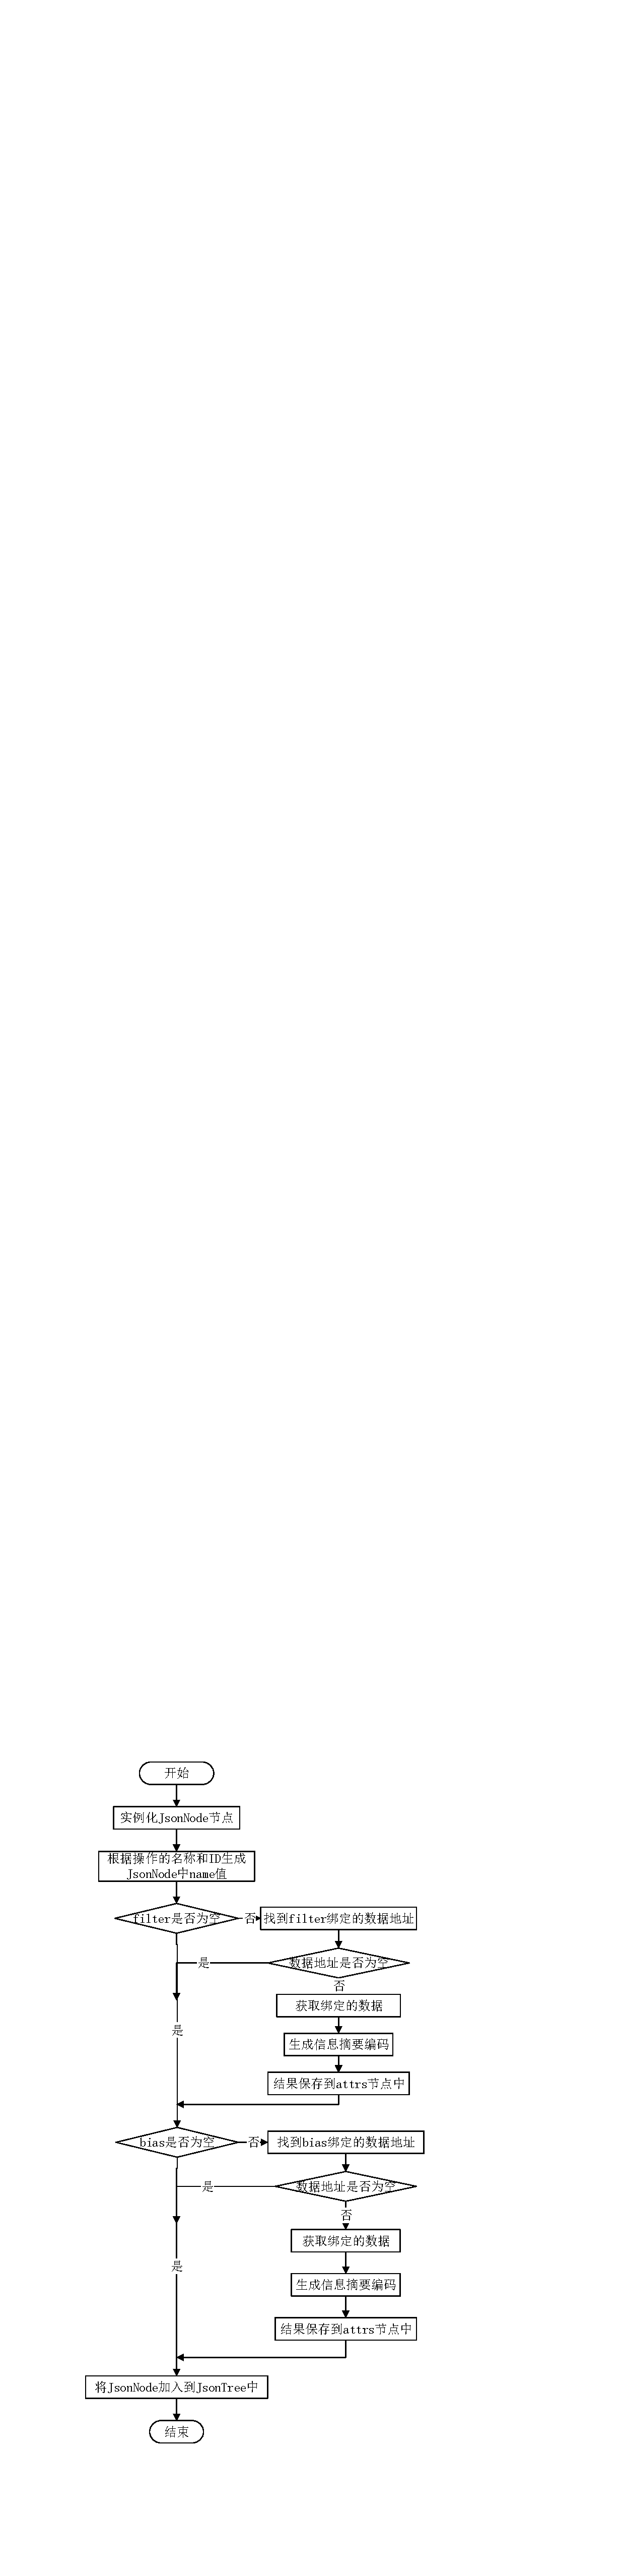
\includegraphics[width=0.5\textwidth]{save_weight_info.pdf}
  }
  \caption{保存结构信息的关键流程图}
  \label{fig:strcut-save-key}
\end{figure}

其实现的关键就是在JsonNode和Operation中保存了指向对方的指针。这样在生成JsonNode的时候可以利用Operation和tensor的关系来判断JsonNode的前驱和后继。如果输入Tensor没有生产者,肯定是神经网络的外部输入,数据在运行时由用户动态填充。

\subsection {保存权值信息}

与保存结构信息相比,保存权值信息就显得相对容易了。因为所有操作的静态书籍不是绑定在filter上就是绑定在bias上,所以所有操作保存权值信息的逻辑都是一样的,如图~\ref{fig:save-weight-info}所示。

首先还是根据操作类型生成唯一的标识name,然后根据是否存在filter和bias以及是否绑定了静态数据分别处理。如果绑定了静态数据,则找到静态数据,生成对应的信息摘要编码,保存到staticdata节点中。

\subsection {保存JsonTree到文件}

将JsonTree保存到文件中,关键就是将JsonTree中包含的JsonNode的内容按照Json的语法规则写入到文件中,。Json语法规则的语法规则如下:
\begin{itemize}
  \item 数据在名称/值对中
  \item 数据由逗号分隔
  \item 花括号保存对象
  \item 方括号保存数组
\end{itemize}
应用到JsonNode,可以分为以下4种情况:
\begin{enumerate}
  \item 当key和content都不为空时,“key”:“content”;
  \item 当key不为空,content为空时,“key”:[childNode] ;
  \item 当key为空,content不为空时,“content”(用于保存前驱节点name的情况);
  \item 当key和content均为空时,{childNode}
\end{enumerate}
在JsonTree的saveToFile函数中,遍历nodes\_,对其中的每个JsonNode调用递归函数saveStemToFile, 递归出口是JsonNode中childNode的大小为0。函数体的主要内容就是判断JsonNode属于上面所述的哪一种情况,然后将内容保存到stringstream中。最后将stringstream写入文件即可。

\section{图信息识别模块设计与实现}
根据JsonTree生成的Josn文件也会占用大量的存储空间,为了节省缓存空间,不直接保存JsonTree生成的Json文件(在调试情况下可以保存下来,方便查看网络结构),而是根据Json文件的内容生成对应的信息摘要编码,保存信息摘要编码后删除对应的Json文件。查找的时候到对应的缓存表中查找是否用相同的信息摘要编码即可。设计到主要的类和方法如图~\ref{fig:graph-info-check}所示。

\begin{figure}[htb]
  \centering
  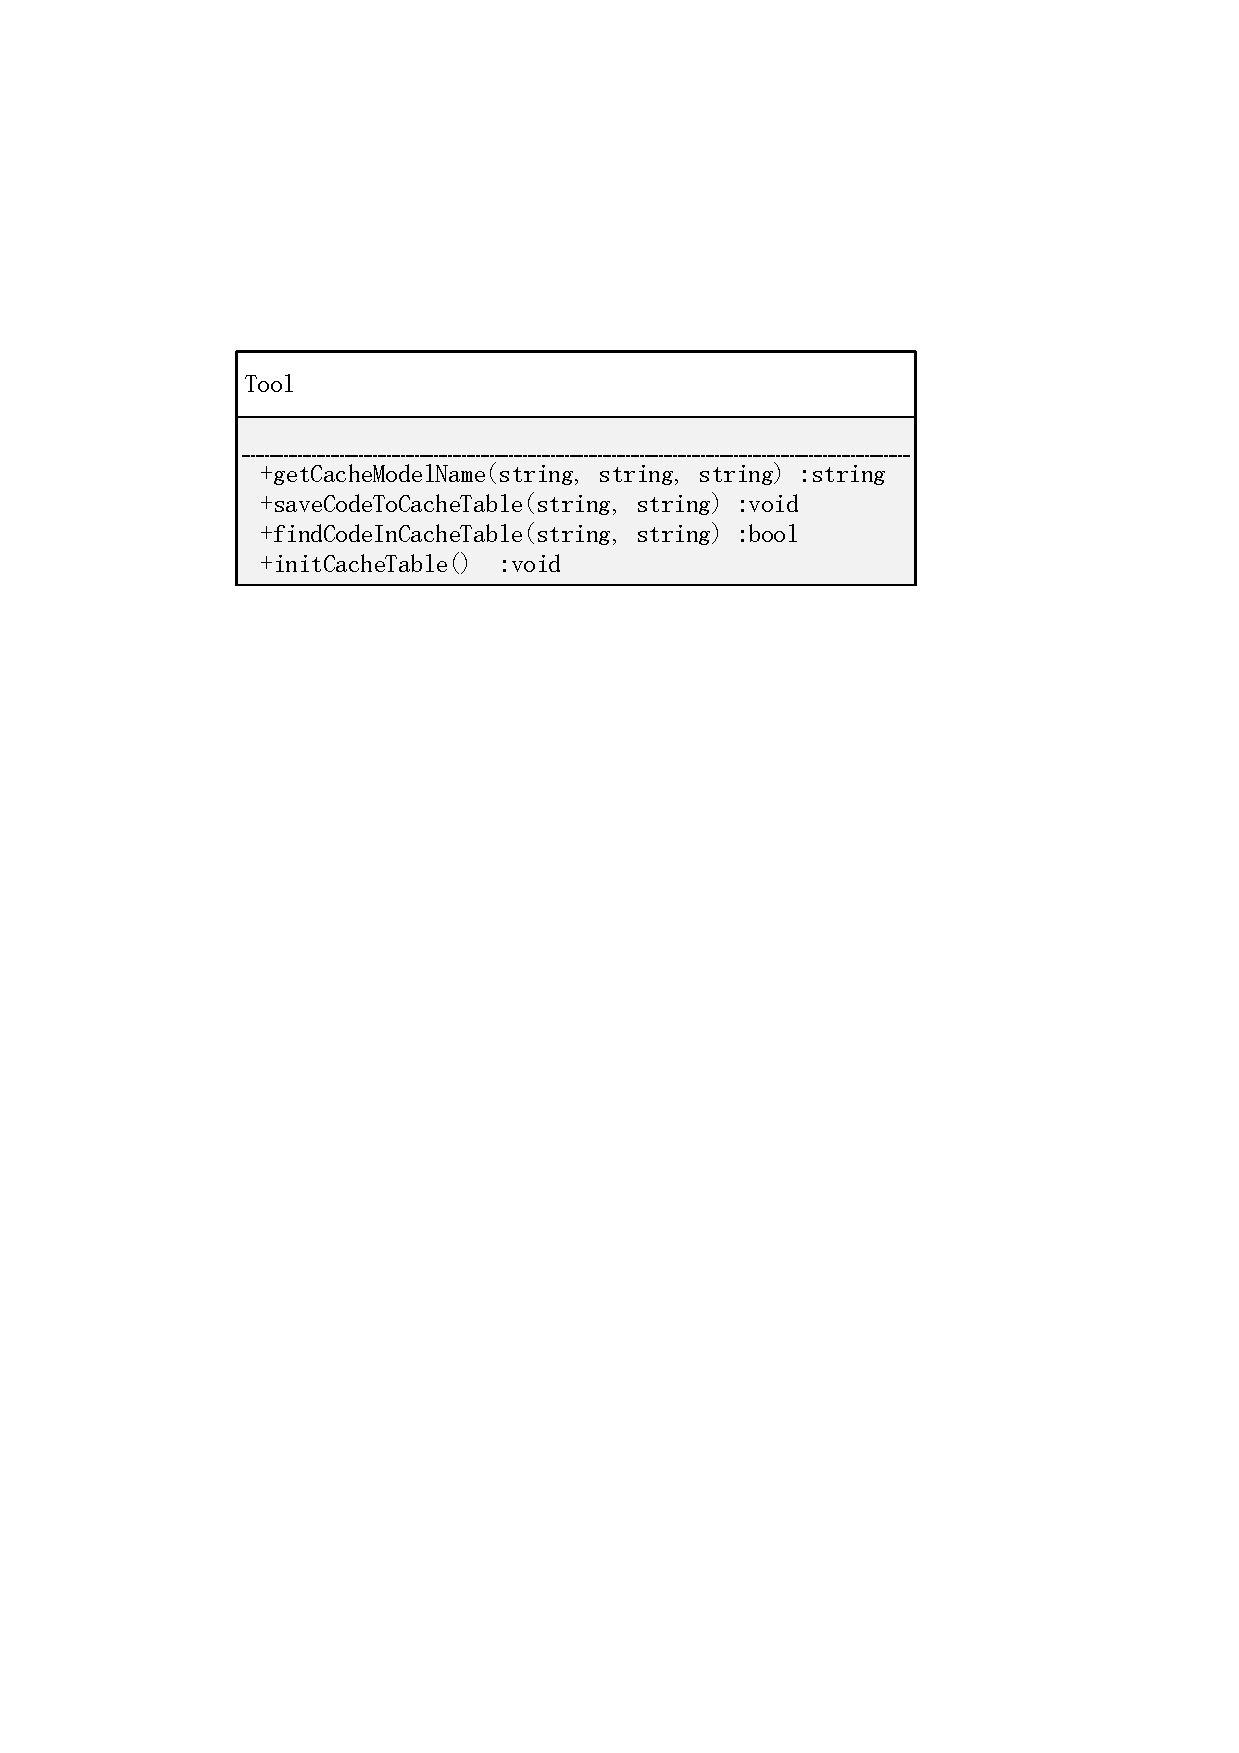
\includegraphics[width=0.5\textwidth]{graph_info_check.pdf}
  \caption{图信息识别模块类图}
  \label{fig:graph-info-check}
\end{figure}

函数功能简介见表~\ref{tab:function-desc-tab}。

\begin{table}[htb]
  \centering\small
  \caption{图信息识别函数功能表}
  \label{tab:function-desc-tab}
  \begin{tabular}{lll}
    \toprule
    函数名      & 功能   & 说明                       \\
    \midrule
    initCacheModel       & 初始化缓存表  & 初始化三张缓存表  \\
    saveCodeToCacheTable & 将摘要编码保存到指定的文件中 &     \\
    findCodeInCacheTable & 在指定的文件中查找指定的摘要编码  & \\
    getCacheModelName & 查找满足要求的指令缓存文件名  & 找到返回文件名,\\
                                                  &&没找到返回空字符串 \\
    \bottomrule
  \end{tabular}
\end{table}

初始化缓存表时初始化三张缓存表,分为是保存环境信息编码的version\_table,保存结构信息编码的struct\_table保存权值信息的data\_table。图识别功能由getCacheModelName函数实现,其流程如图~\ref{fig:get-cache-model}所示。

\begin{figure}[htb]
  \centering
  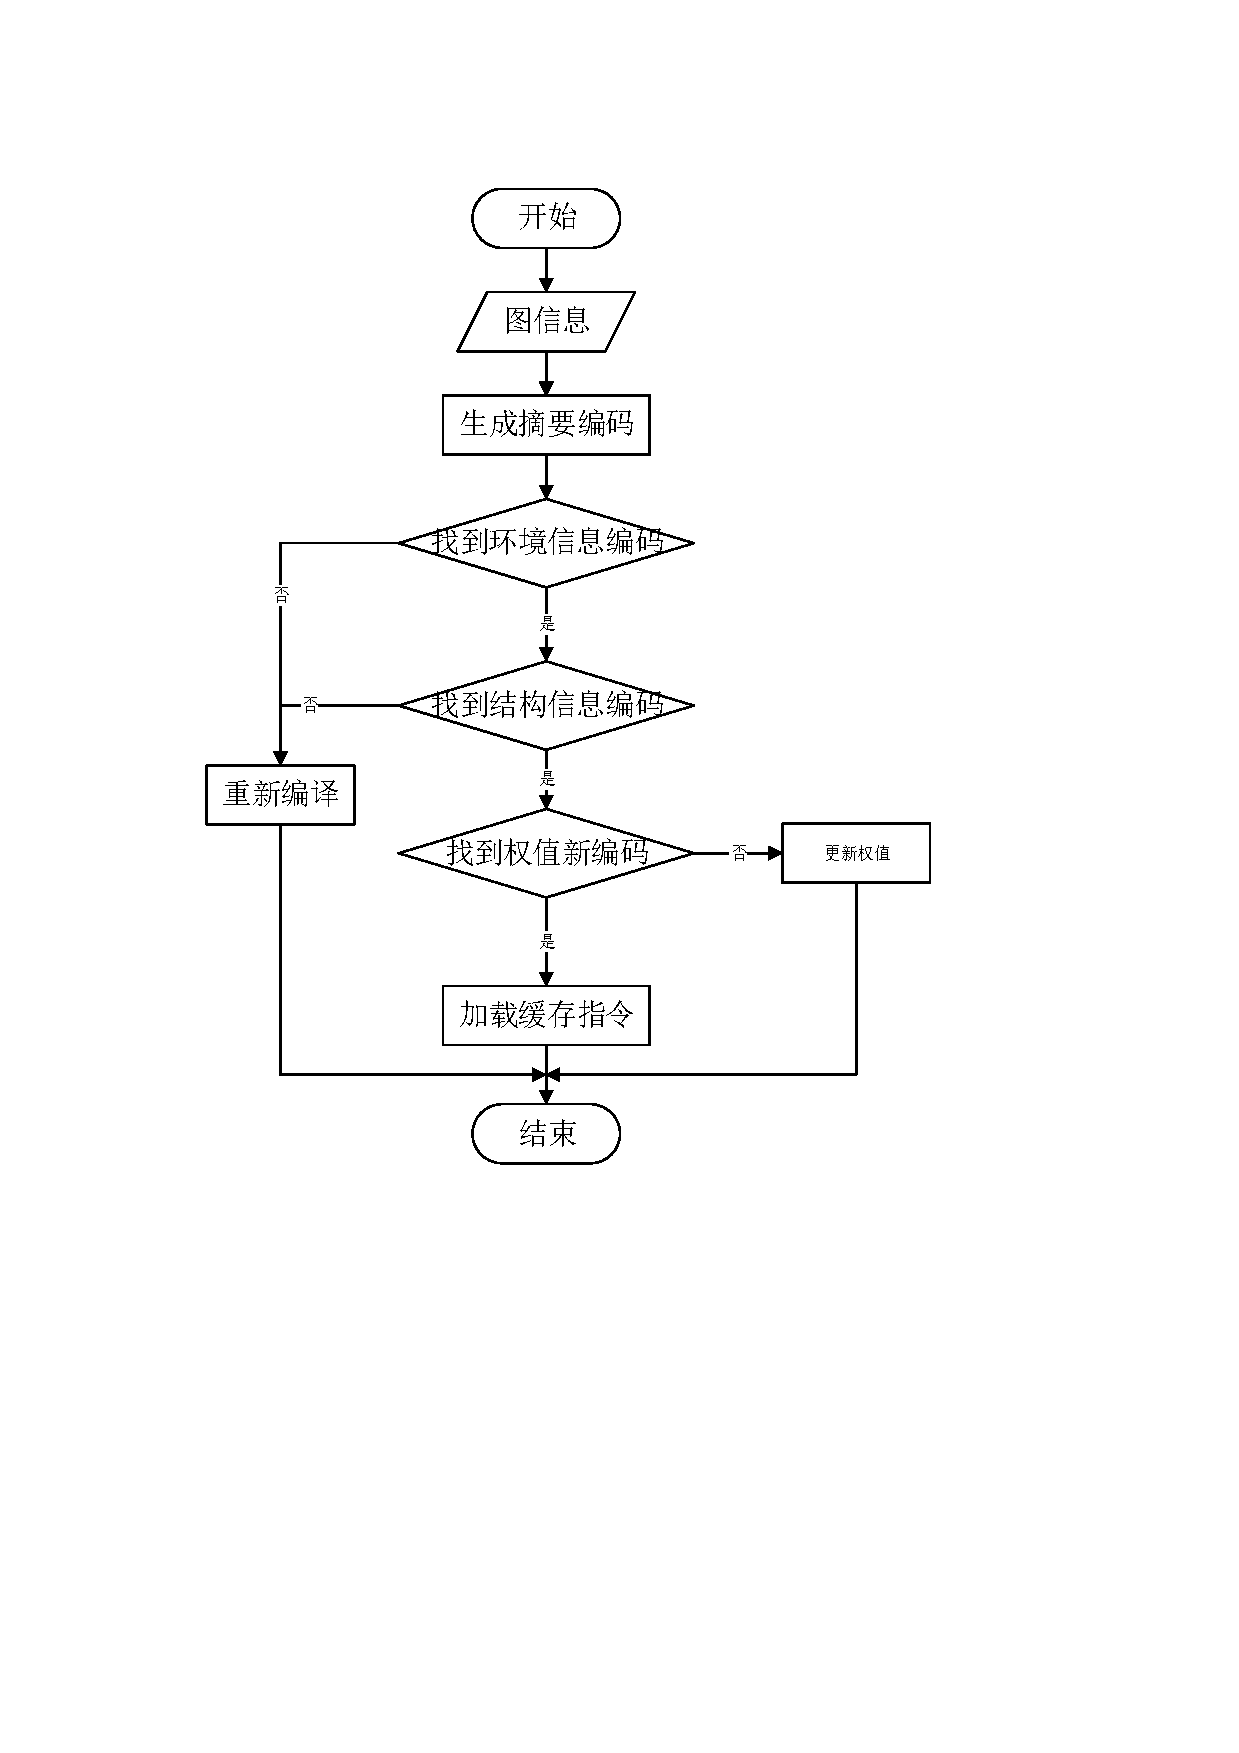
\includegraphics[width=0.5\textwidth]{get_cache_model.pdf}
  \caption{图信息识别模块类图}
  \label{fig:get-cache-model}
\end{figure}

比较的时候只先根据信息摘要算法对三部分信息生成对应的摘要编码,然后在version\_table中查找是否有当前的环境信息编码,没有代表编译环境发生了变化,需要重新编译;如果当前环境信息摘要编码存在于环境信息表,则继续在struct\_table中查找结构信息摘要编码,如果没找到,重新编译;如果找到则继续在data\_table中查找权值信息摘要编码,如果找到,则说明已经缓存了一份满足条件的指令,直接加载这份指令即可,如果只是权值信息编码没有找到,则拿一份结构相同的指令进行权值替换,也不需要重复编译。

\section{指令保存和加载模块设计与实现}
该模块设计的主要任务是将kernel离线保存到文件然后在需要的时候从文件中解析出之前保存的kernel。由于不同平台的kernel可以有很多不同的结构和设计方式,并且kernel的详细结构和功能对本模块的影响不大。所以本模块将淡化kernel的详细设计,而将重点放在如何实现指令的保存和加载上。类之间的关系如图~\ref{fig:load-cache-class}所示。

\begin{figure}[htb]
  \centering
  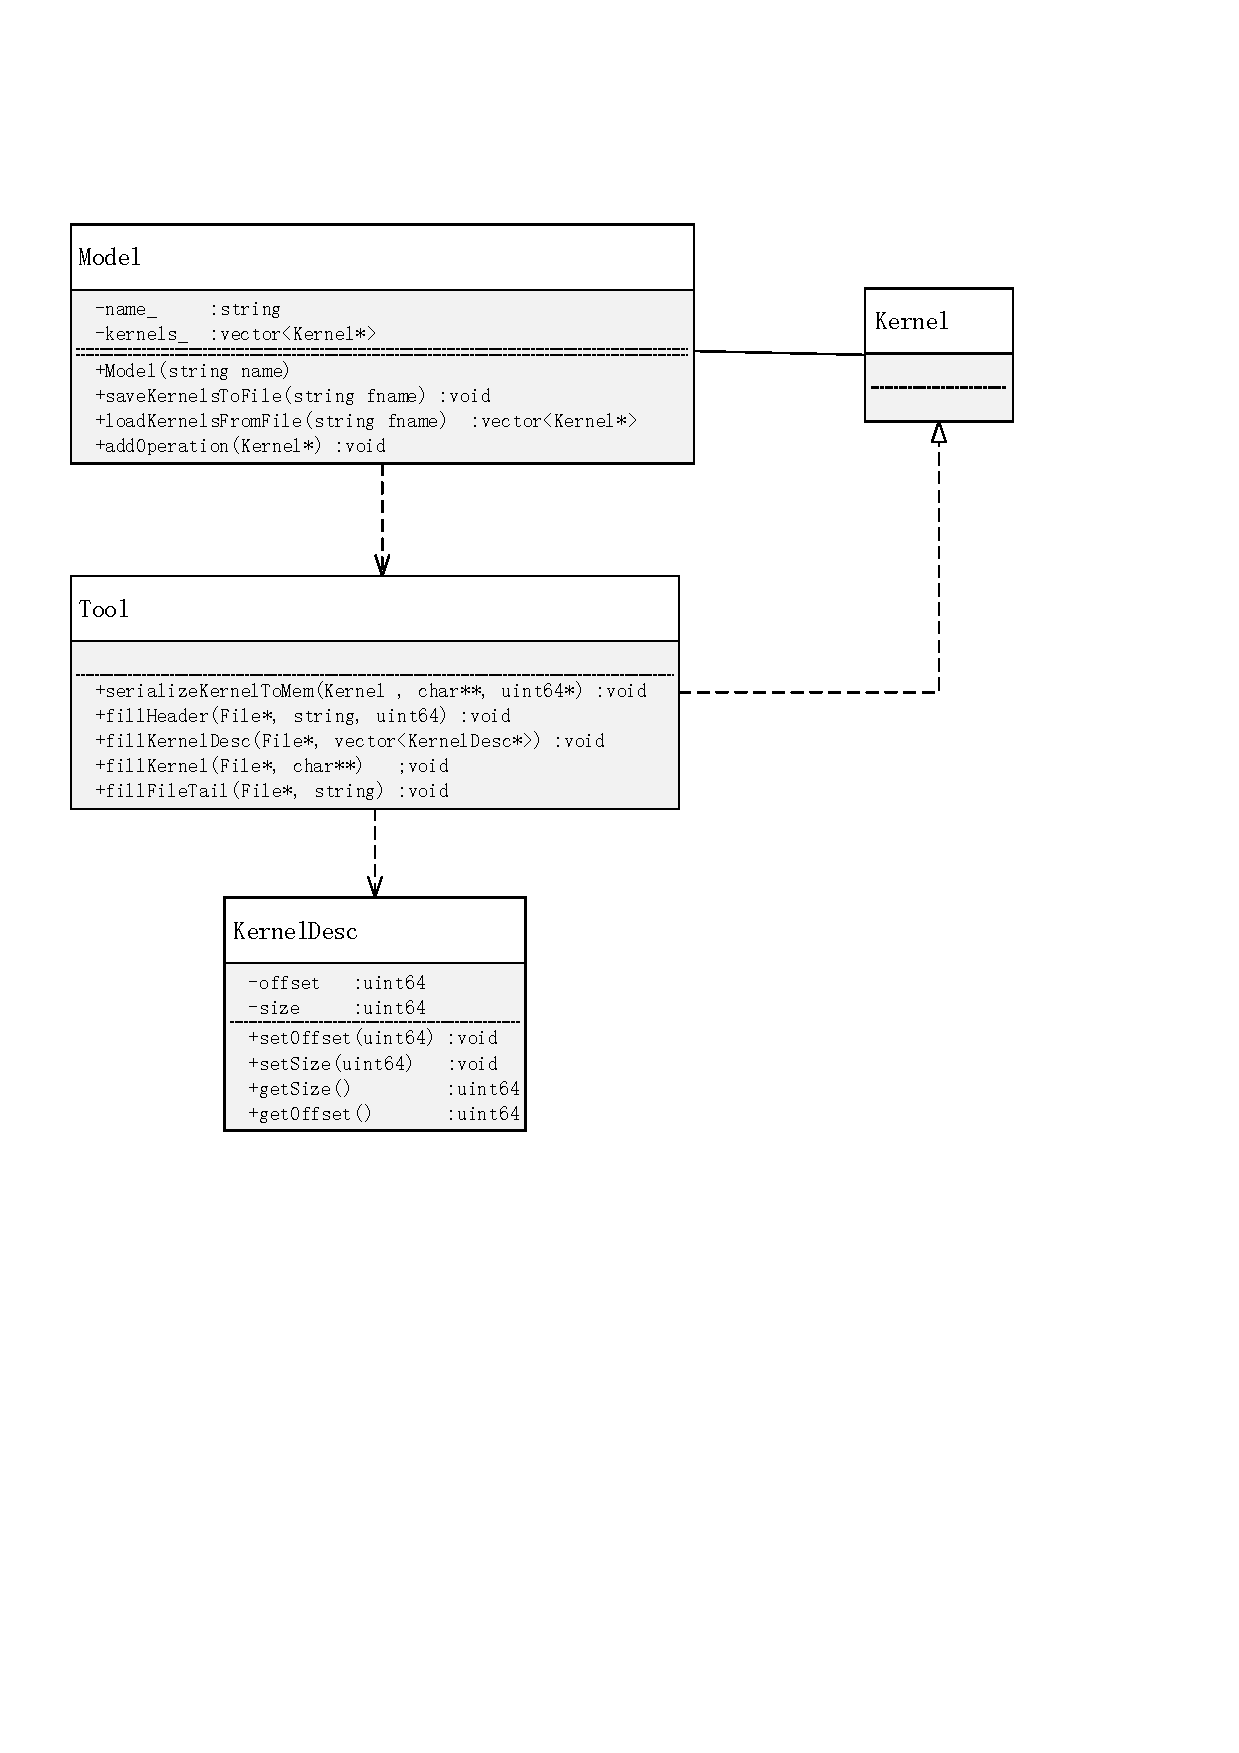
\includegraphics[width=0.5\textwidth]{load_cache_class.pdf}
  \caption{指令保存和加载模块类图}
  \label{fig:load-cache-class}
\end{figure}


该模块的实现主要由4个类组成:Model、Kernel、Tool、KernelDesc。Model作为保存离线模型和加载离线模型的入口;Tool主要实现模型内容的填充。这两个类的主要函数功能见表~\ref{tab:model-tool-function-list}。

\begin{table}[htb]
  \centering\footnotesize
  \caption{Model和Tool主要接口说明}
  \label{tab:model-tool-function-list}
  \begin{tabular}{llll}
    \toprule
    类名        & 函数名     & 功能      & 说明            \\
    \midrule
    Model      & saveKernelsToFile    & 将多个kernel保存到离线文件中 &  \\
               & loadKernelsFromFile  & 从离线文件中加载kernel &    \\
               & addOperation         &向kernels\_中添加kernel & \\
    \midrule
    Tool       & fillKernelDesc & 填充离线模型文件目录部分 & \\
               & fillKernel   & 填充离线模型文件中kernel的内容 & \\
               & fillFileTail & 填充离线模型文件的结尾  & 填入文件前面所有\\
                                                    &&&内容对应的MD5码 \\
               & fillHeader & 填充离线模型文件头 & 传入模型名称和需要    \\
                                                &&&保存的kernel数量\\
               & serializeKernelToMem & 将kernel序列化后 & 传入需要系列化的kernel,\\
                                      &&保存到内存中     & 返回序列化后的字符串地 \\
                                                       &&&址和返回序列化后占用 \\
                                                       &&&空间大小  \\
               
    \bottomrule
  \end{tabular}
\end{table}


在指令缓存的过程中离线模型的文件名,模型名,文件标识符,校验码等信息由程序自动生成,对用户不可见。文件名和模型名都根据之前生成的信息摘要编码组成。文件名=环境信息编码+结构信息编码+权值信息编码,模型名=结构信息编码+权值信息编码,结构如图~\ref{fig:model-name-struct}所示。


\begin{figure}[htb]
  \centering
  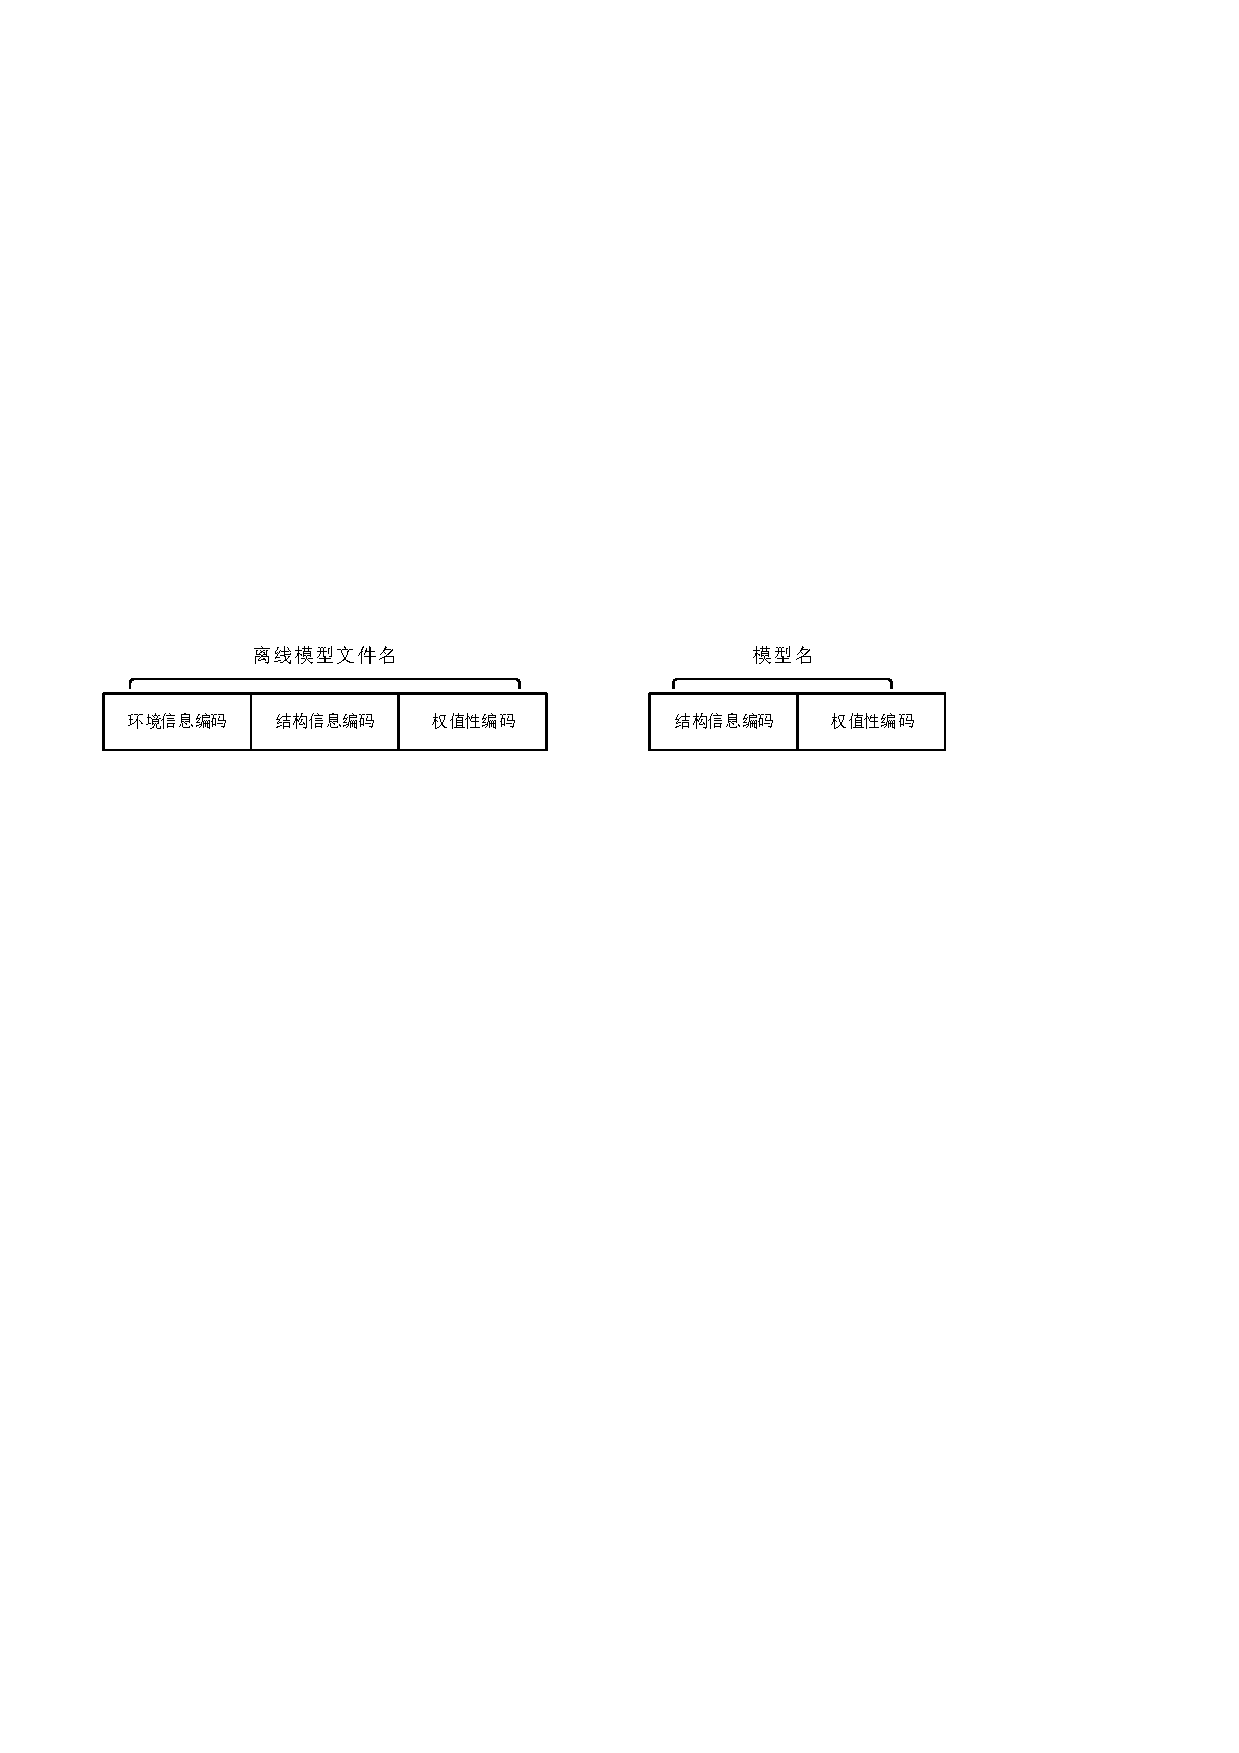
\includegraphics[width=0.8\textwidth]{model_name_struct.pdf}
  \caption{文件名和模型名组成示意图}
  \label{fig:model-name-struct}
\end{figure}

Kernel序列化后的内容就是一个字符串,占用存储空间大小和字符串中字符的数量相关。保存指令通过函数saveKernelsToFile实现,流程如图~\ref{fig:kernel-process}-(a)所示。

\begin{figure}[htb]
  \centering
  \subfigure[保存流程图]{
  \label{fig:save-kernel-process}
  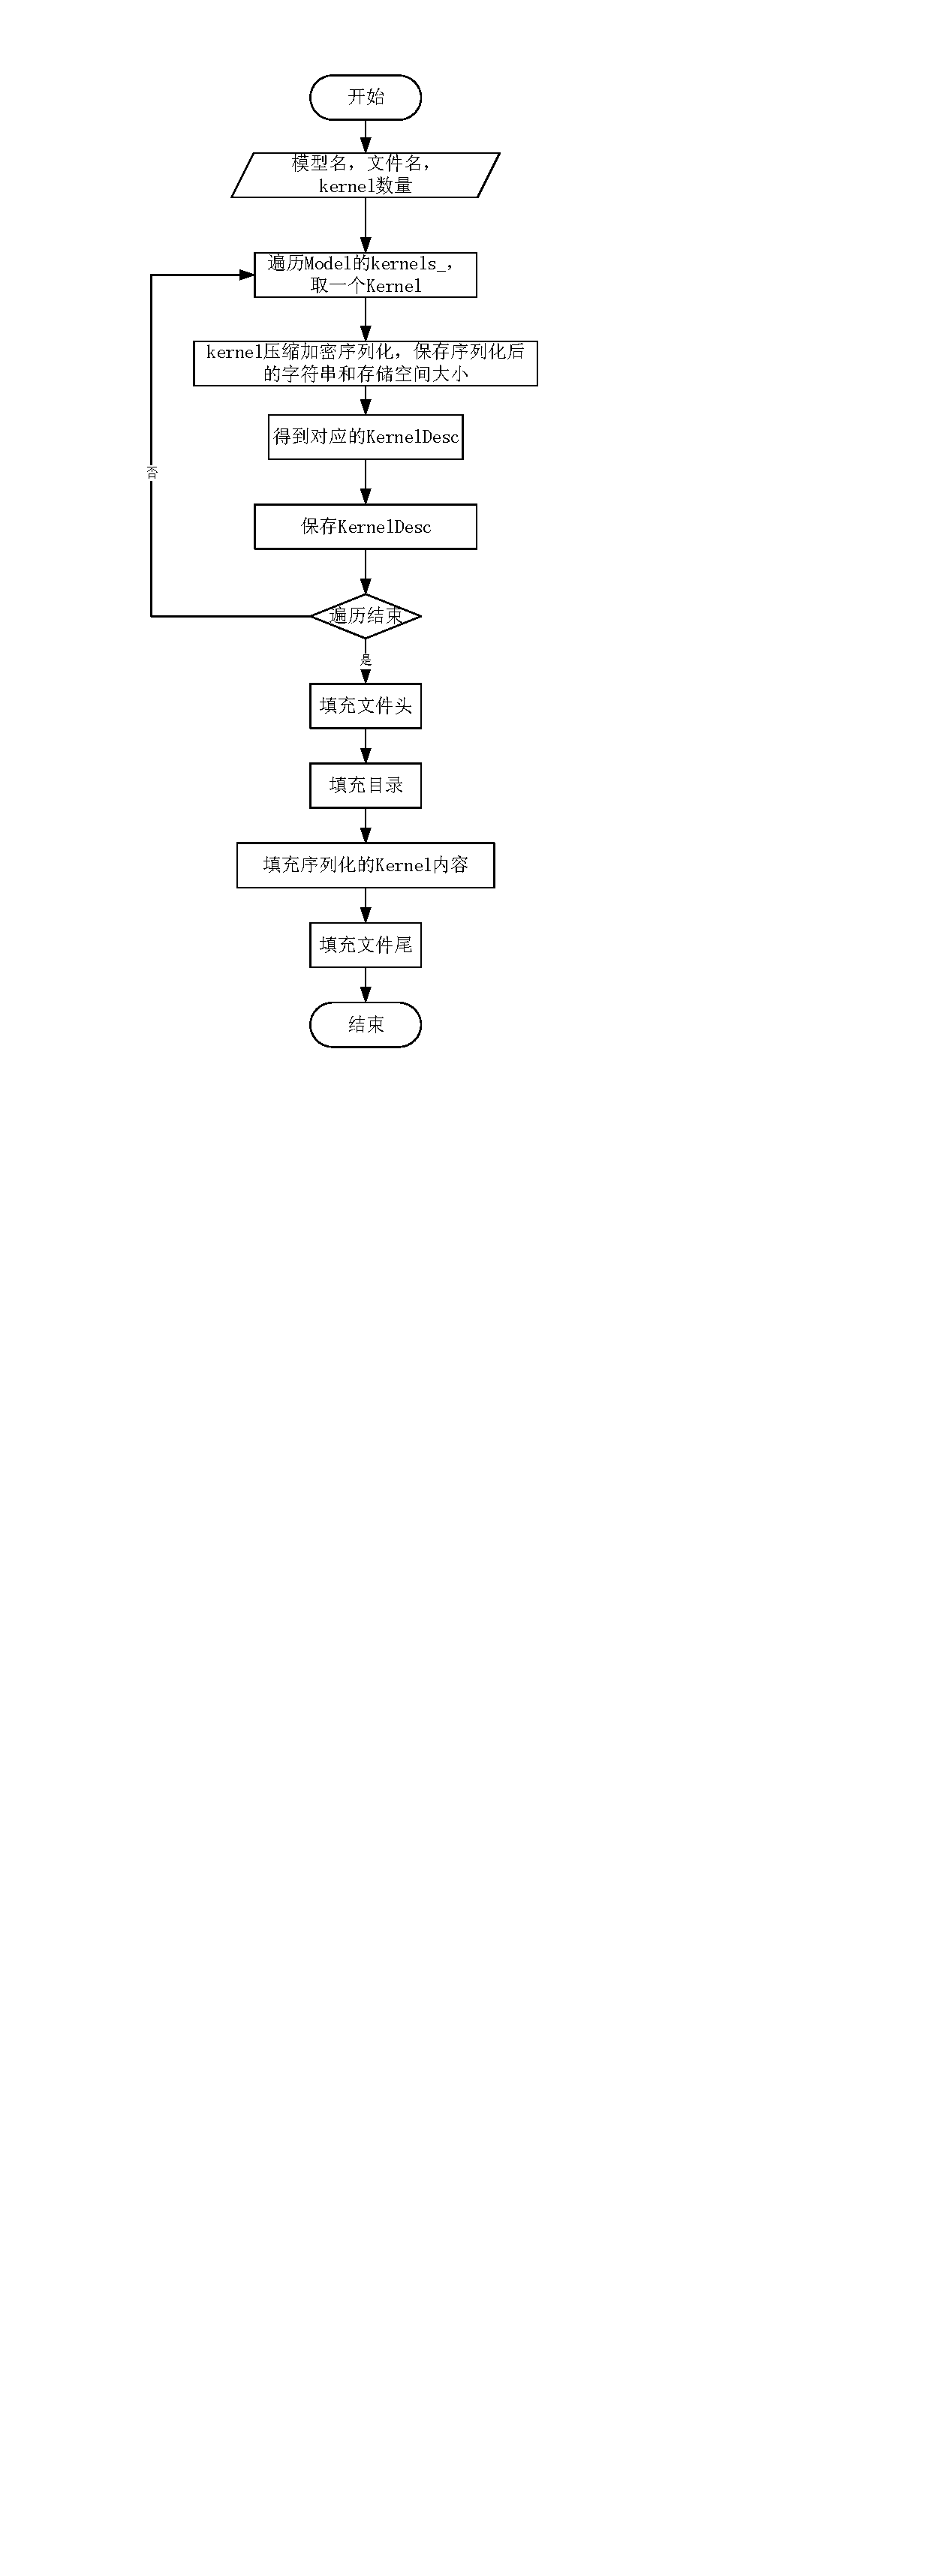
\includegraphics[width=0.45\textwidth]{save_kernel_process.pdf}
  }
  \subfigure[加载流程图]{
  \label{fig:load-kernel-process}
  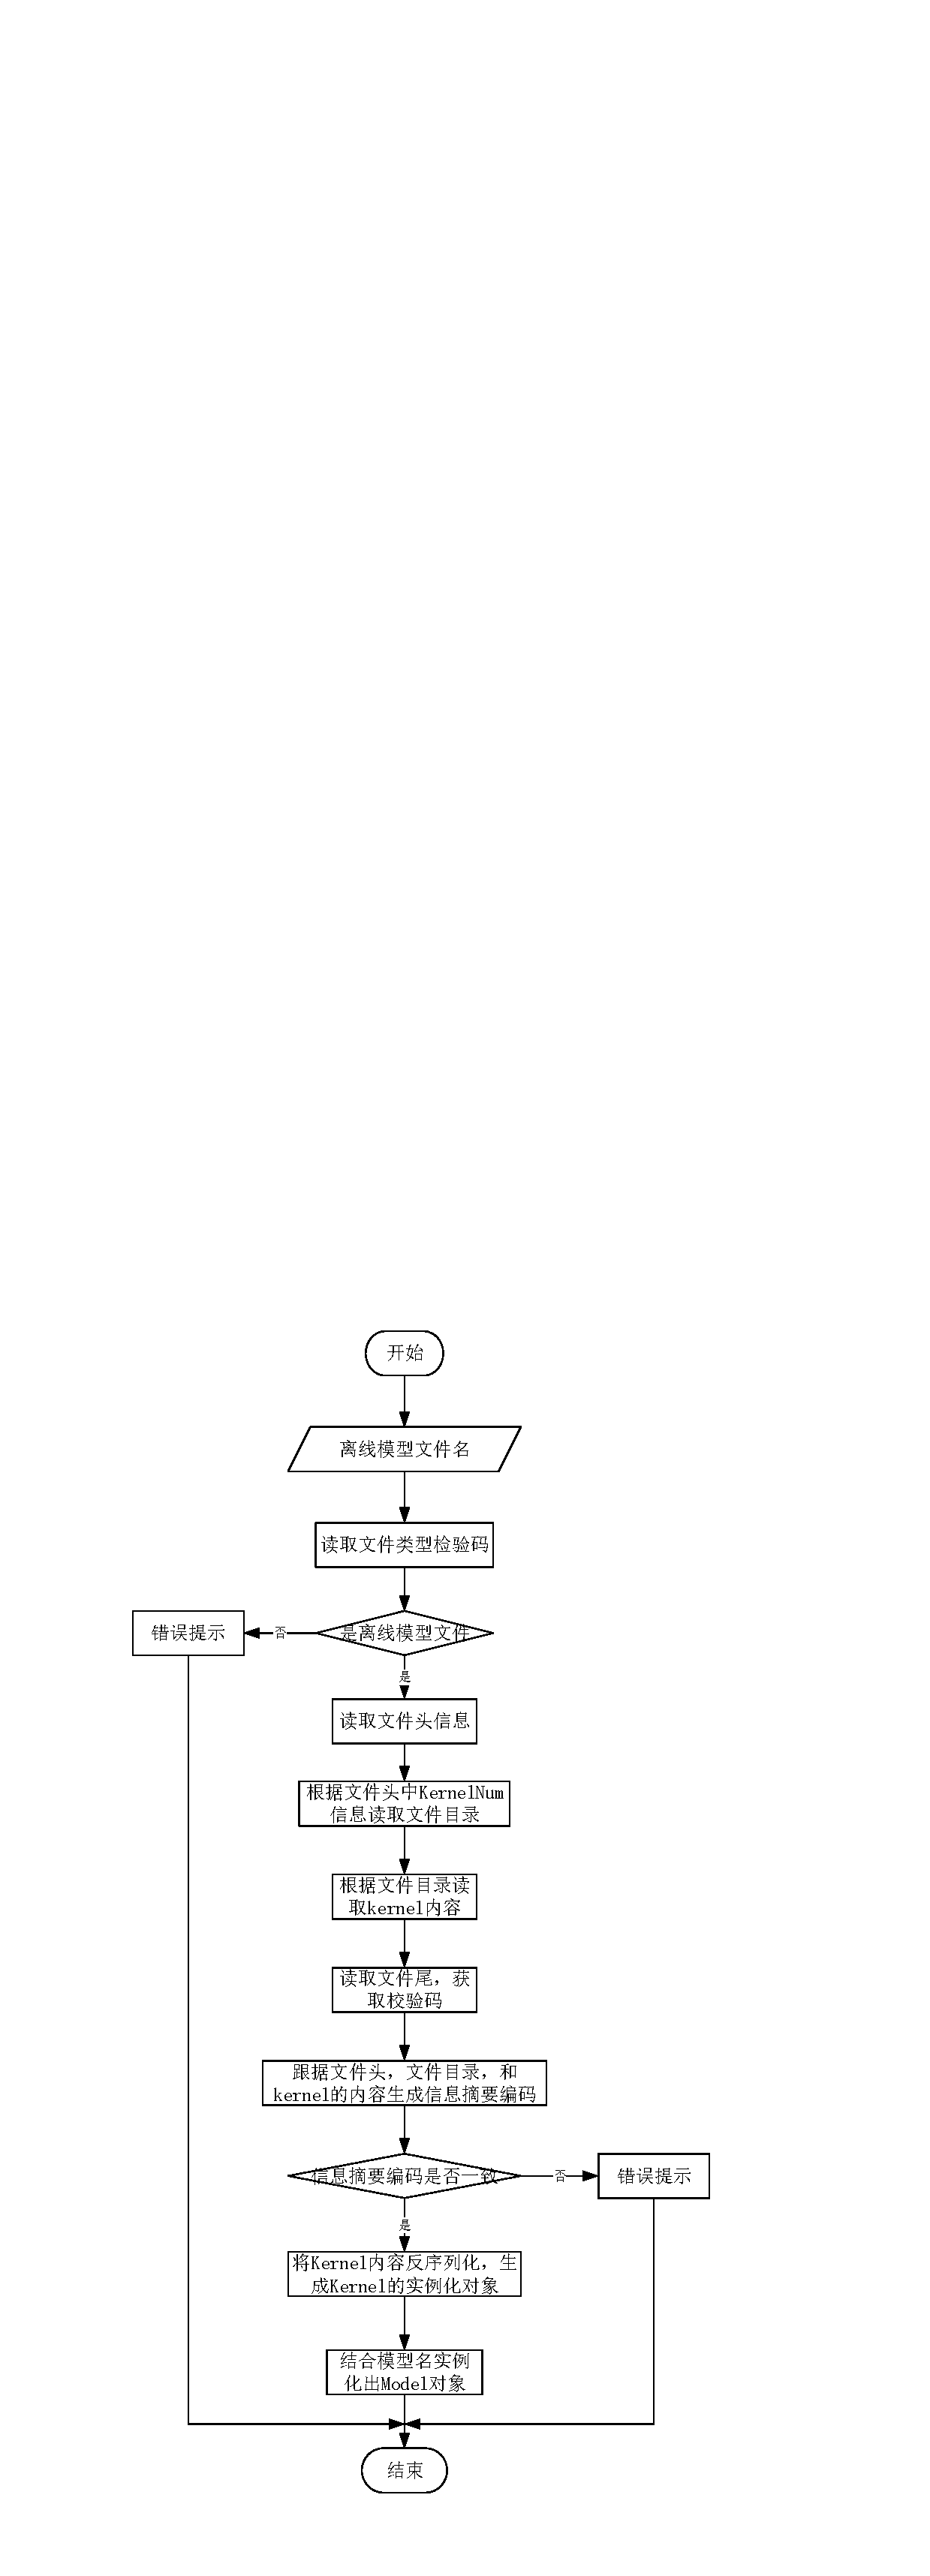
\includegraphics[width=0.4\textwidth]{load_kernel_process.pdf}
  }
  \caption{kernel保存和加载流程图}
  \label{fig:kernel-process}
\end{figure}

保存指令的步骤如下:
\begin{enumerate}
  \item 拿到Model中所有的Kernel
  \item 对每一个Kernel按一定压缩和加密算法进行压缩和加密,得到二级模型(序列化后的字符串)和占用存储空间大小,并用两个数组分别保存;
  \item 根据二级模型大小和偏移,生成对应的KernelDesc并保存到数组中。
  \item 根据二级模型总大小,文件头大小,文件尾大小,目录大小计算出模型文件总大小,将文件总大小、模型数量、模型名、校验码,版本号等文件头信息写入文件。
  \item 遍历保存KernelDesc的数组,将offset和size信息依次写入文件,完成文件目录的填充;
  \item 遍历保存二级模型内容和大小的数组,结合二级模型的内容依次写入文件中,完成文件模型内容的填充
  \item 根据文件头,文件目录和文件模型的内容生成一个信息摘要编码,写入到文件最后,完成文件尾的填充
\end{enumerate}
加载指令是保存指令的逆过程,通过函数loadKernelFromFile完成,流程如图~\ref{fig:kernel-process}-(b)所示。

加载指令的步骤如下:
\begin{enumerate}
  \item 根据传进来的离线模型文件名打开离线模型文件。
  \item 读取文件中文件类型校验码的内容,判断是否是离线模型文件,如果不是,则给出错误提示信息后退出;如果是,则继续进行下一步。
  \item 读取固定大小的文件头内容。
  \item 根据文件头中模型的数量读取文件目录的内容。
  \item 根据文件目录的内容,读取出每个离线模型的内容。
  \item 最后读取文件尾的校验码。
  \item 根据文件头,目录,离线模型的具体内容生成新的信息摘要编码,与文件尾保存的信息摘要编码比较,如果不一致,说明文件损坏,给出提示后退出;如果一致,说明文件完好,继续执行下一步。
  \item 发序列化离线模型的内容,生成Kernel的实例化对象。
  \item 结合模型名,生成Model的实例化对象。
\end{enumerate}
生成kernel的实例化对象之后将kernel送给模型执行器,继续执行kernel的计算过程。

\section {权值替换模块设计与实现}
在神经网络应用中,神经网络结构相同,权值(为了方便起见,这里将filter和bias统称为权值)不同的情况经常发生,为了尽可能的避免神经网络的重复编译(编译阶段耗费大量的时间)。当遇到结构相同,权值数据不同的情况下,我们可以通过权值替换的手段来避免二次编译。

权值替换的原理就是拿一份结构相同的已经编译好的离线模型文件,替换掉其中的权值数据。由于网络模型结构相同,替换数据之后和新编译生成的指令完全一样,所以执行结果不会产生差异。

实现过程中涉及到的类及其方法如图~\ref{fig:weight-replace-class}所示。

\begin{figure}[htb]
  \centering
  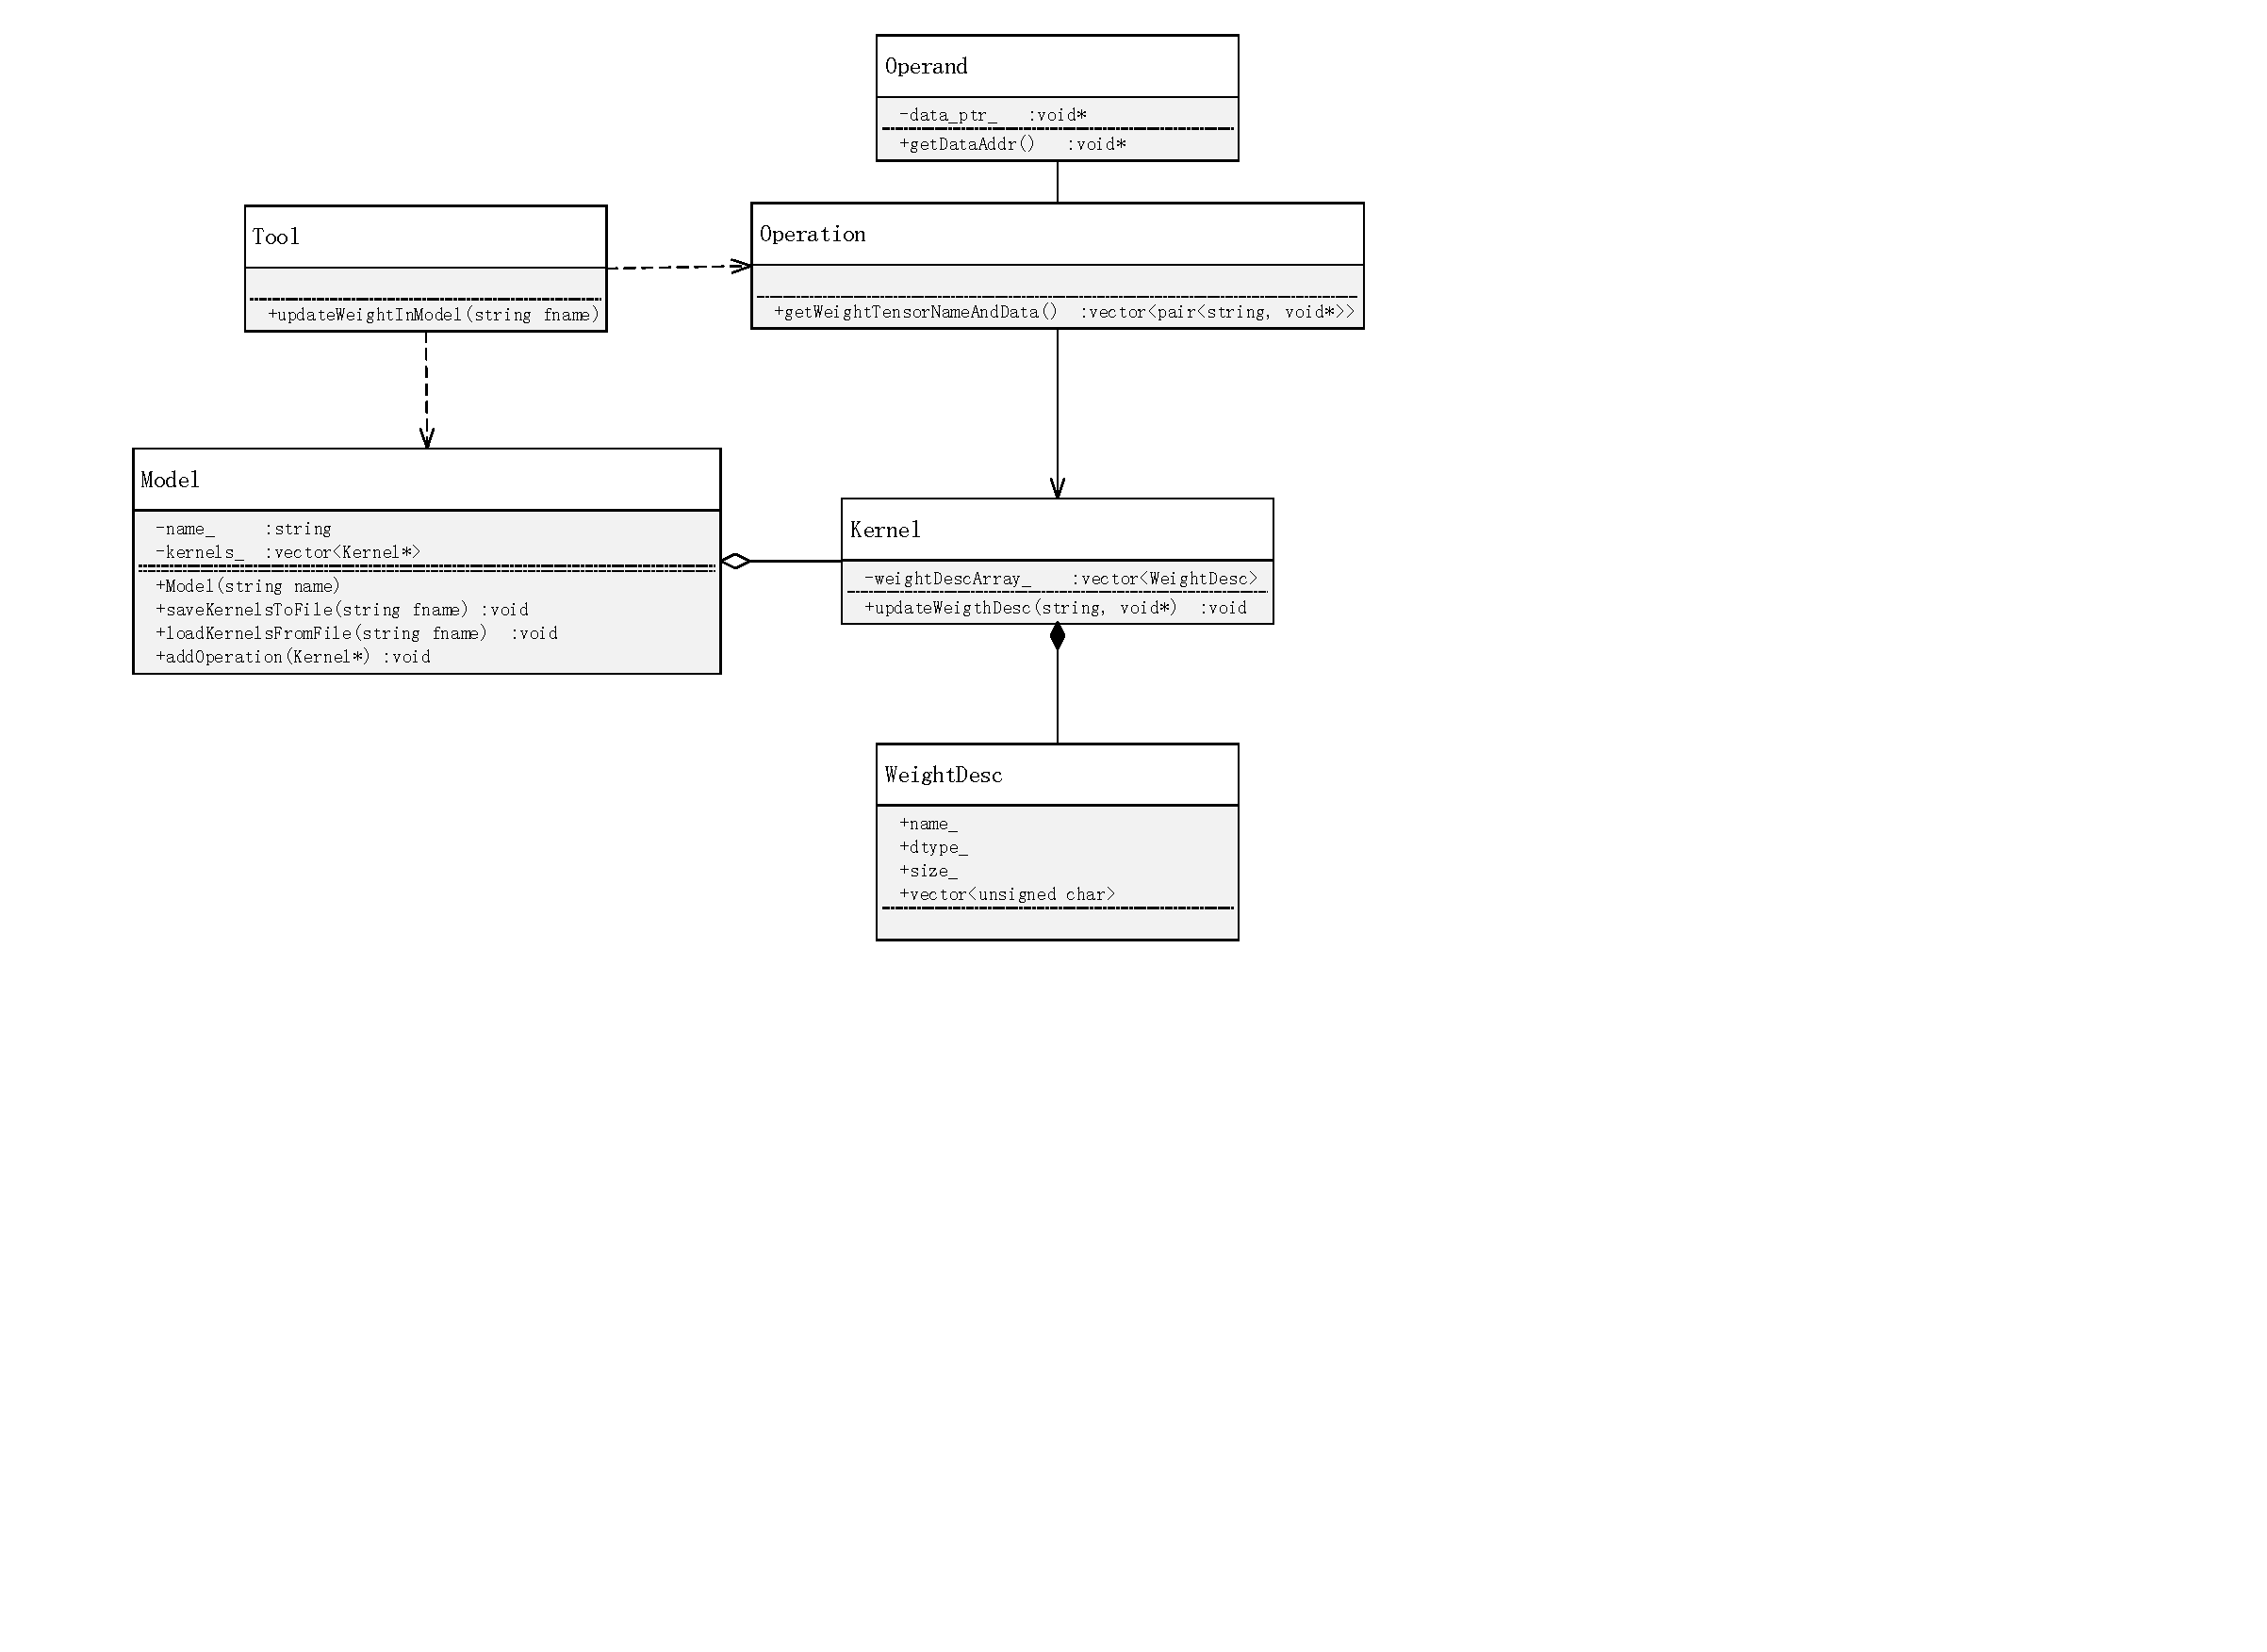
\includegraphics[width=0.8\textwidth]{weight_replace_class.pdf}
  \caption{权值替换模块类图}
  \label{fig:weight-replace-class}
\end{figure}

其中WeightDesc用于保存权值信息,包括对应的Tensor名称、数据类型、数据个数、和实际数值,为了方便存储和读取各种类型的数据,用unsigned char类型存储实际数据,取值的时候根据数据类型,将unsigned char类型转换为对应的数据。主要函数说明见表~\ref{tab:weight-replace-function-list}。

\begin{table}[htb]
  \centering\small
  \caption{权值替换模块主要函数说明}
  \label{tab:weight-replace-function-list}
  \begin{tabular}{lll}
    \toprule
    函数名        & 功能     & 函数说明                 \\
    \midrule
    Tool:updateWeightInModel  & 更新指定离线模型 &将多个kernel保存到 \\
                              &文件中的权值数据   离线文件中\\
    \midrule
    Operand:getDataAddr & 获取Tensor绑定 &如果没有绑定数据,\\
                        &数据的地址   & 则返回默认值nullptr  \\
    \midrule
    Operation: & 获取操作中所有Filter和Bias &如果是融合操作,会返 \\
    getWeightTensorNameAndData  & 类型的Tensor的名称 & 回图中所有操作的Filter\\
                      &和绑定的数据地址 &和Bias类型Tensor的 \\
                      &                &名称和绑定的数据地址 \\
    \midrule
    Kernel: updateWeightDesc  & 更新kernel中指定 & 第一个参数是Tensor名 \\
                              & Tensor绑定的数据 & 称,第二个参数新数据地址 \\
    \bottomrule
  \end{tabular}
\end{table}

权值替换实现的流程如图~\ref{fig:weight-replace-process}所示。

\begin{figure}[htb]
  \centering
  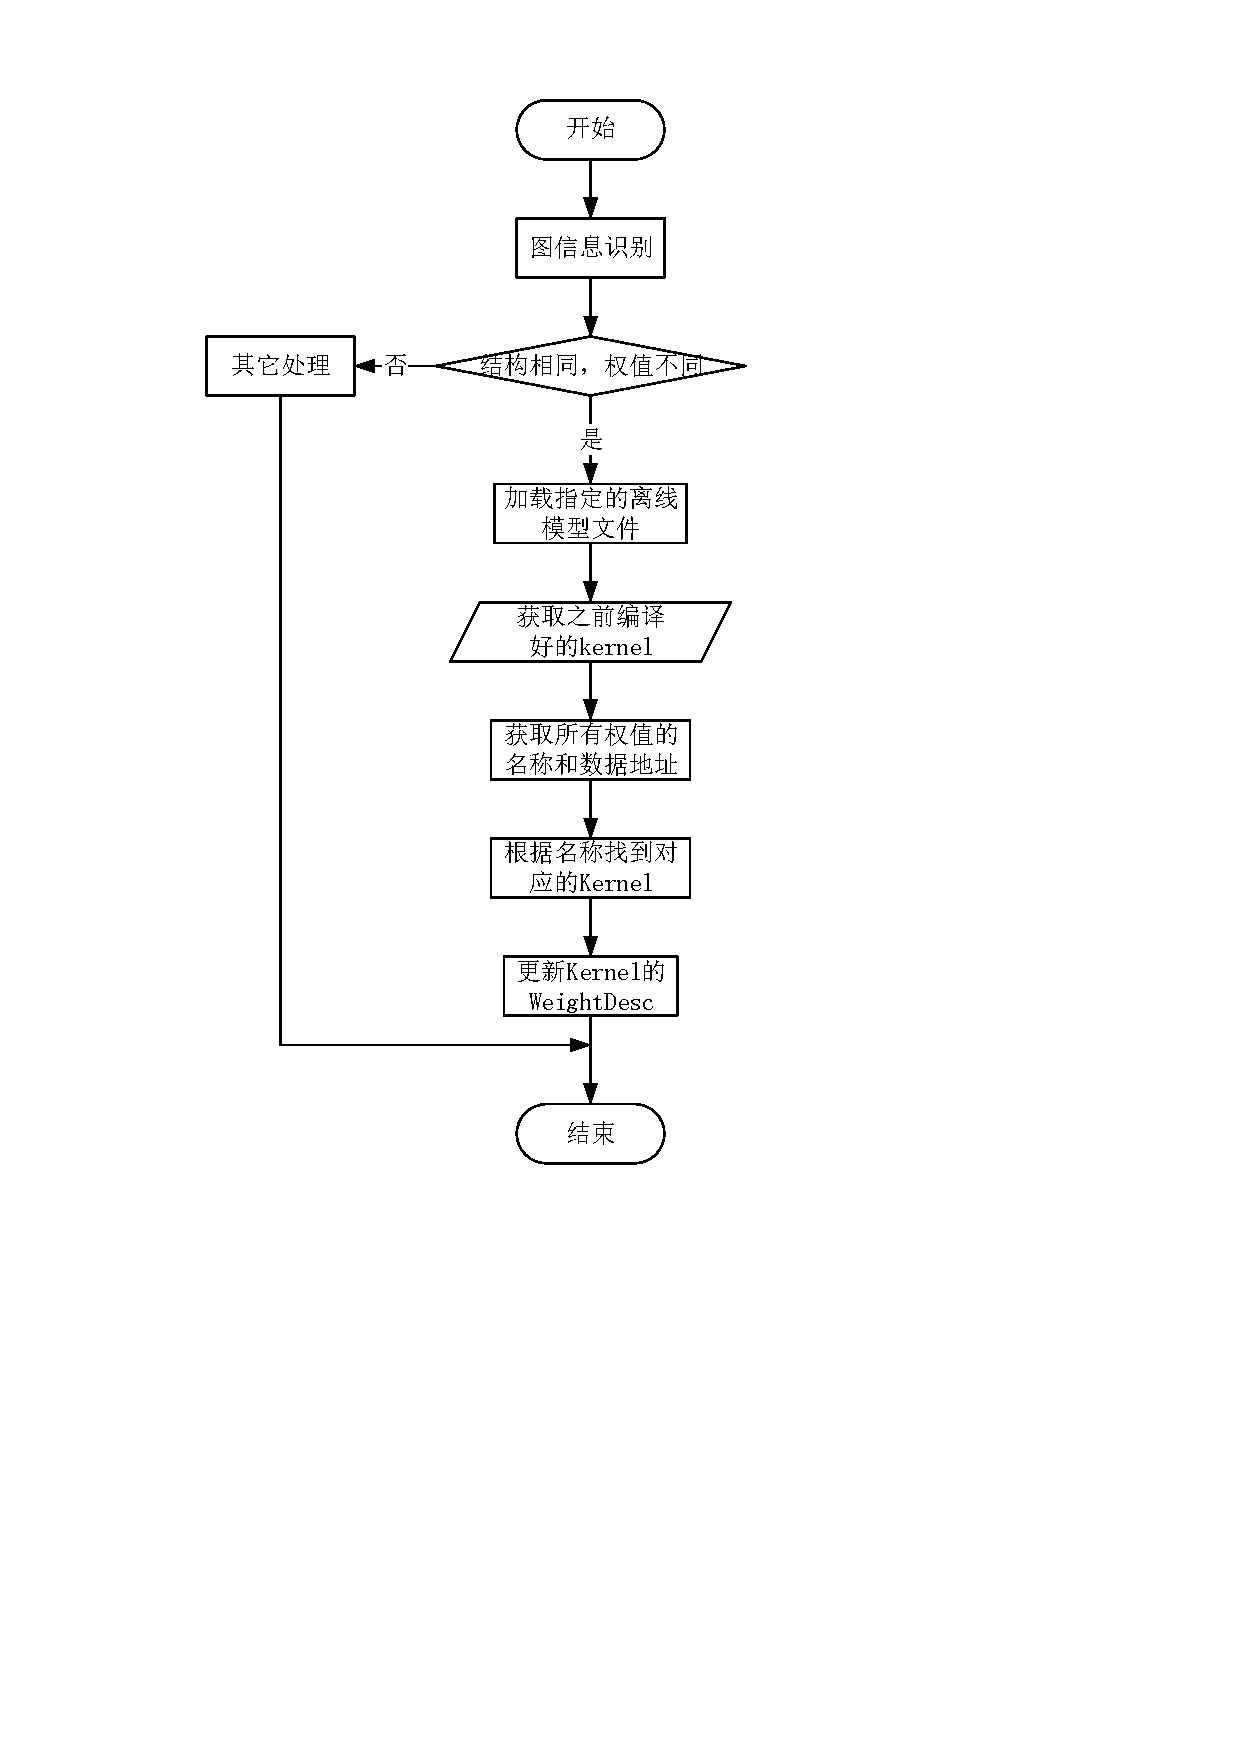
\includegraphics[width=0.3\textwidth]{weight_replace_process.pdf}
  \caption{权值替换模块流程图}
  \label{fig:weight-replace-process}
\end{figure}

如果在图信息识别模块中识别出是结构相同而权值不同的情况则进行权值替换。首先加载一份结构相同的离线模型文件,解析文件,生成对应的kernel对象;然后查找出所有绑定权值信息的Tensor的名称和绑定的数据地址;之后根据tensor的名称查找出对应的kernel对象,更新kernel中对应Tensor的数据。

权值信息更新完毕后,将kernel送入模型执行器,并保存一份新的离线模型文件,更新权值信息缓存表。

\section {指令替换模块设计与实现}

指令替换模块是指令缓存的子功能,当缓存空间不足时进行指令替换,删除旧指令文件,保存新指令文件。
为了支持用户友好性,用环境变量MODEL\_CACHE\_DISABLE来控制是否开启指令缓存,默认值为0,默认情况下开启指令缓存功能,值为1时关闭指令缓存功能;用环境变量MODEL\_CACHE\_MAXSIZE来设定缓存空间大小,只有当MODEL\_CACHE\_DISABLE的值为0时设置该环境变量才有效。当指令缓存关闭时,编译阶段不会执行计算图信息保存、识别,权值替换等流程。

指令替换采用先进先出(First In First Out、FIFO)的原则,符合缓存功能的定义也符合深度学习的使用场景,特别是在训练阶段,为了达到满意的效果,经常需要不断的调整权值信息。此时根据先进先出的原则,可以大概率的编译重复编译。

为了实现指令替换,我们还需要用一个环境变量ACHE\_SIZE\_LEFT来保存当前缓存空间的剩余量。替换流程如图~\ref{fig:cache-replace-process}所示。

\begin{figure}[htb]
  \centering
  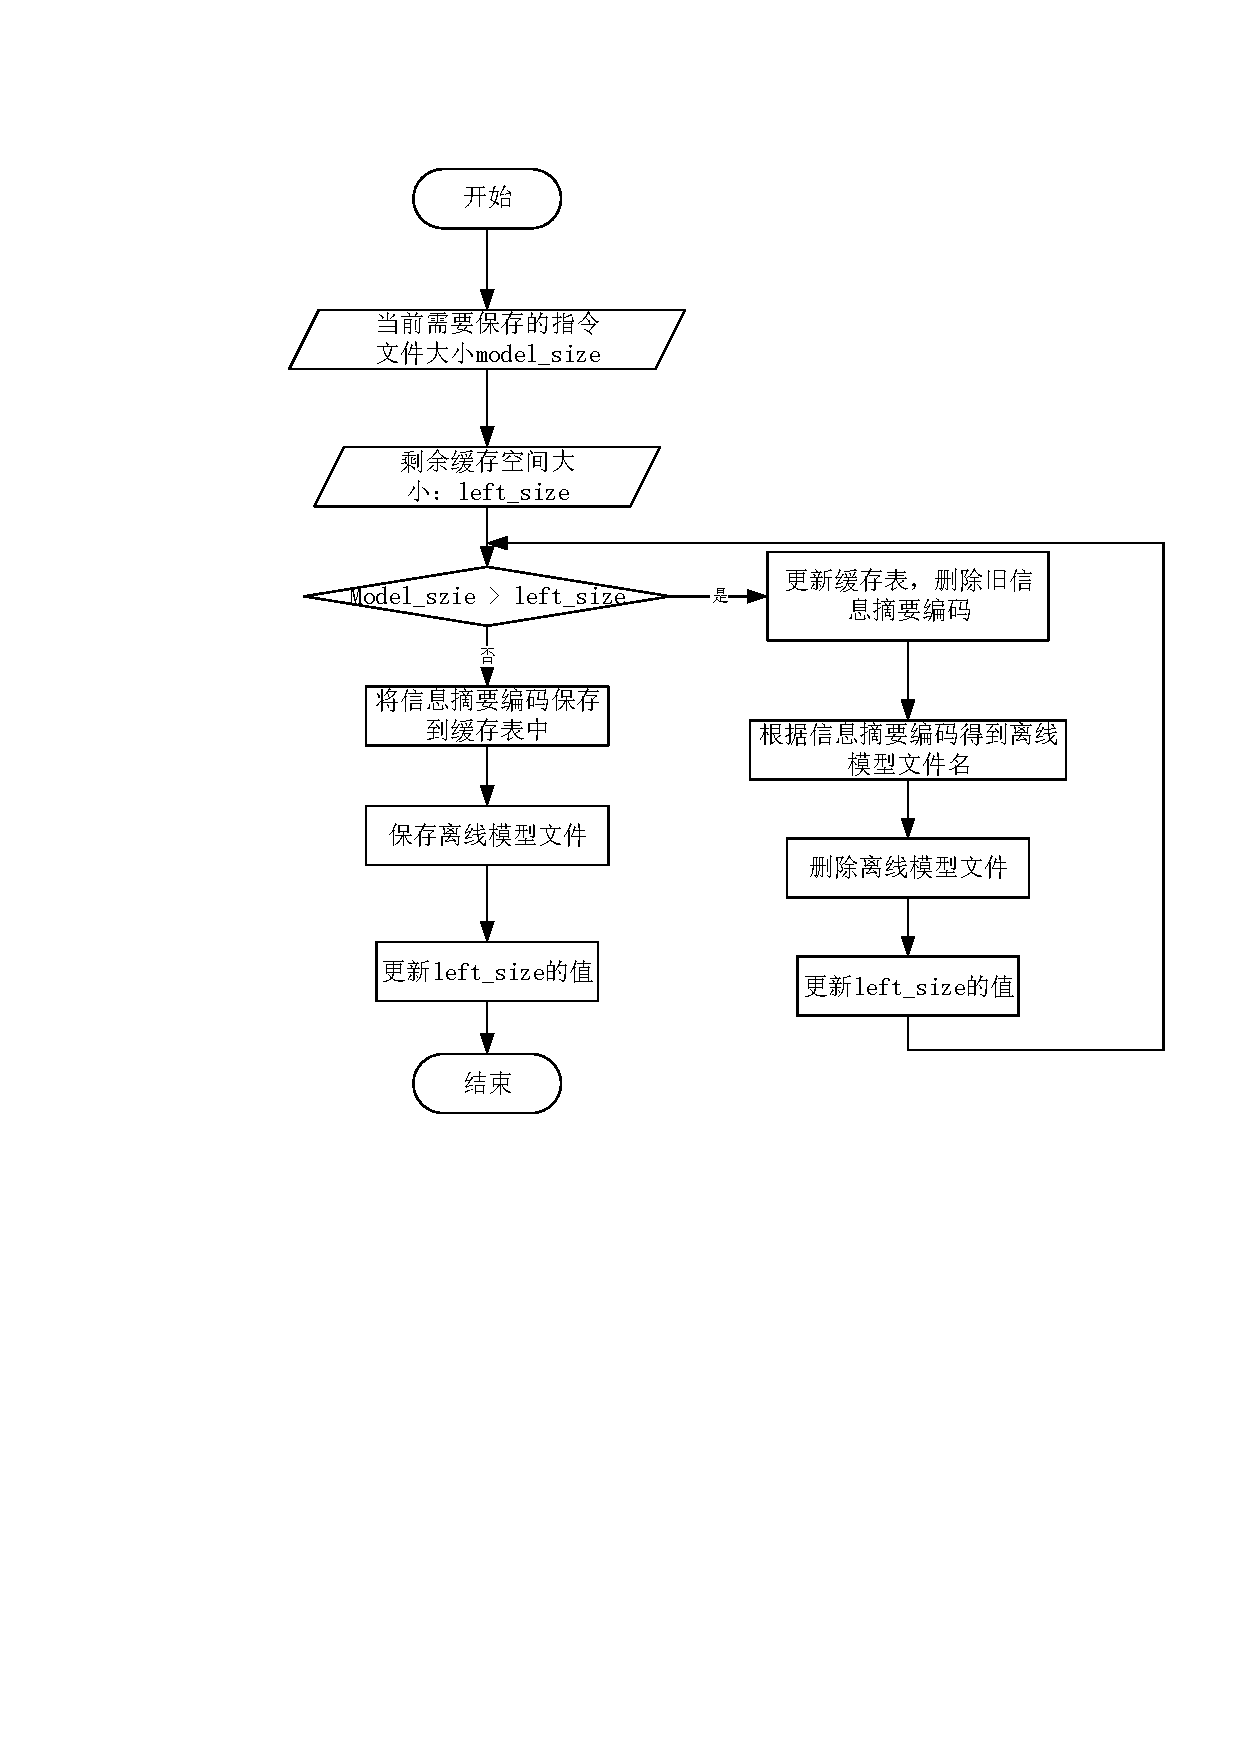
\includegraphics[width=0.6\textwidth]{cache_replace_process.pdf}
  \caption{替换离线模型流程图}
  \label{fig:cache-replace-process}
\end{figure}

首先判断当前缓存的剩余空间是否充足,如果剩余空间充足,则直接更新缓存表,保存新的离线模型文件,更新剩余空间的值即可;如果剩余的空间不充足,则删除最旧的离线模型文件,更新缓存表,更新剩余空间的值,重新比较剩余空间是否满足,如果不满足则继续删除离线文件的过程,直到剩余空间大小满足为止。

\section {权值量化模块设计与实现}
权值量化通过利用低精度的int8类型的数据来表示量化后的float型的数据从而达到模型压缩的目的。事实上,在对精度要求并不是十分苛刻的情况下,量化神经网络不仅能压缩神经网络的空间,更能提高神经网络的推理和训练速度。
为了用户友好性,由用户通过环境变量ENABLE\_QUANTIFY\_MODEL来控制是否开启权值量化。默认值为false,不开启权值量化功能;当环境变量值为true时,开启权值量化功能。类图如~\ref{fig:weight-quant-class}所示。

\begin{figure}[htb]
  \centering
  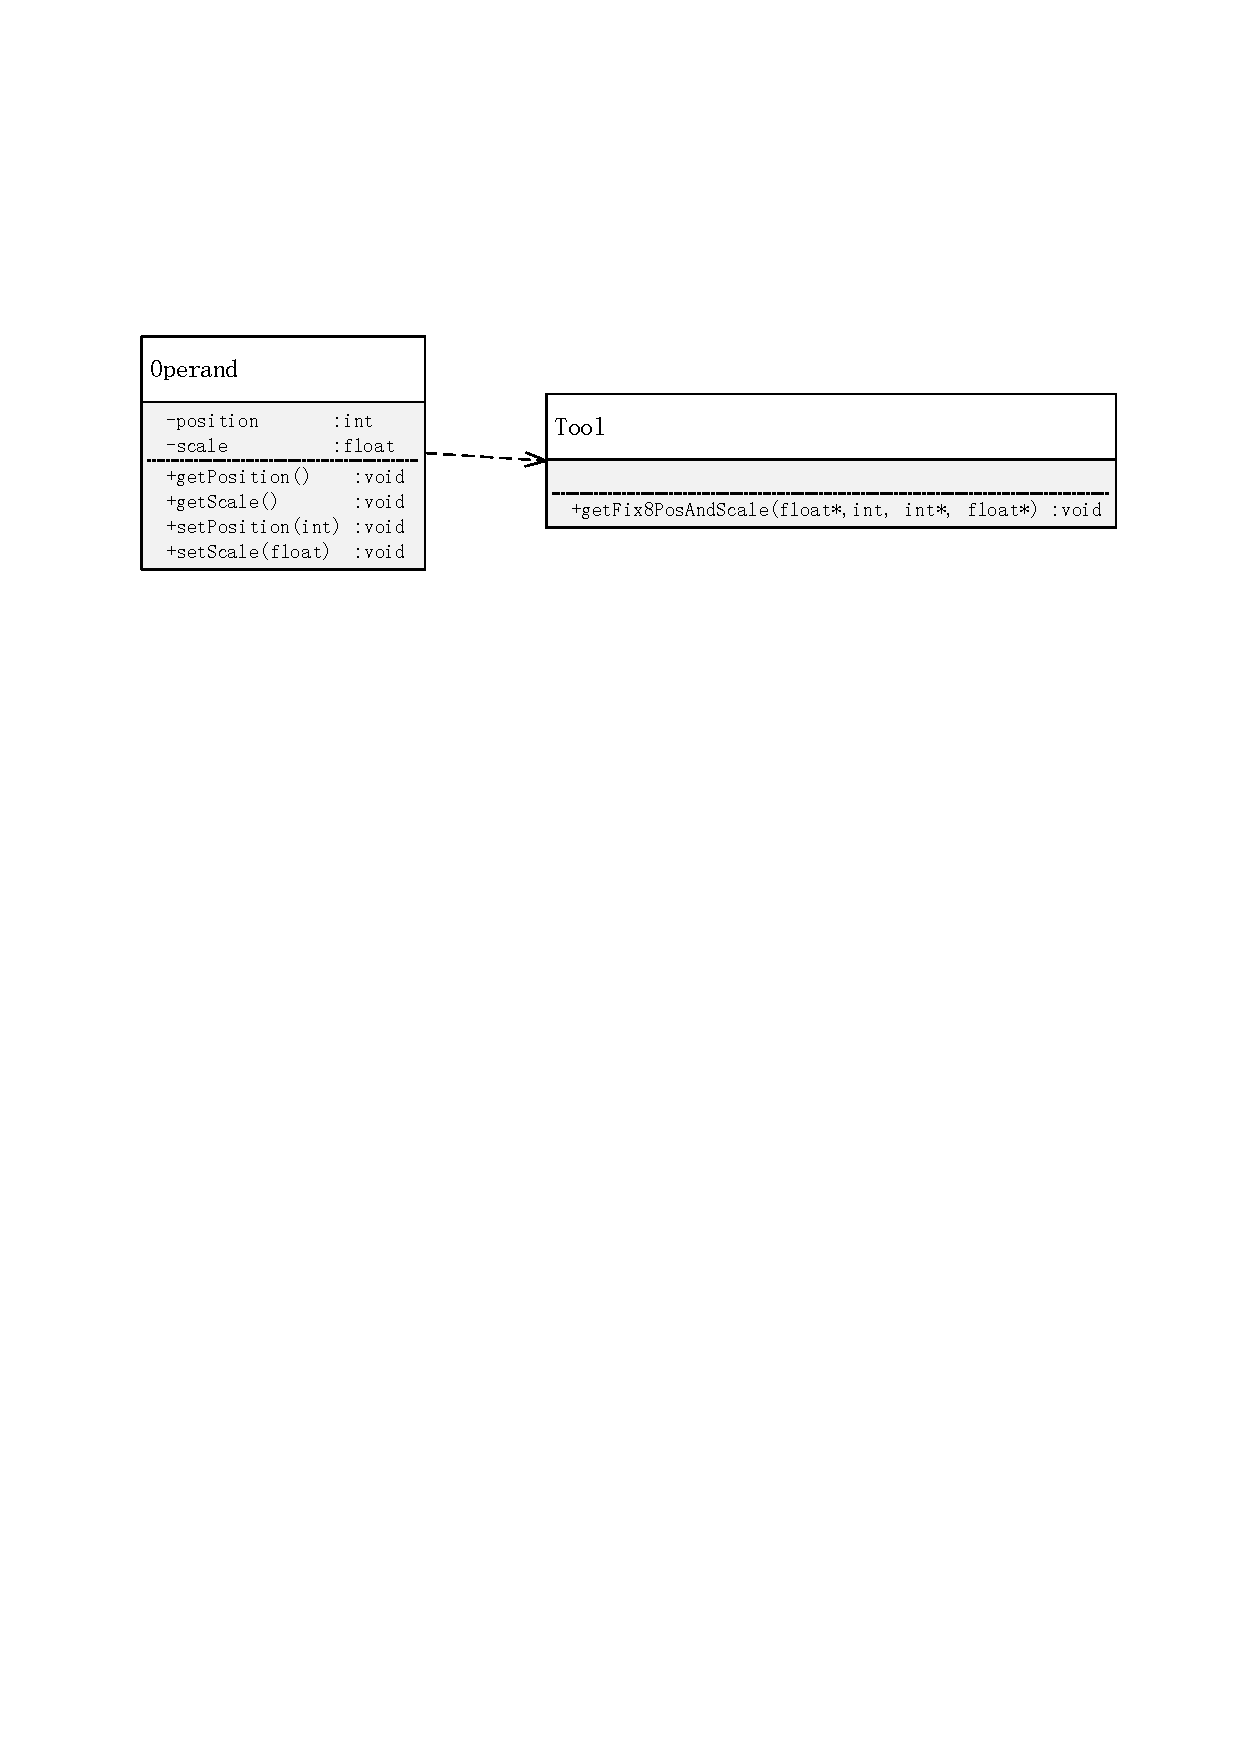
\includegraphics[width=0.9\textwidth]{weight_quant_class.pdf}
  \caption{权值量化模块类图}
  \label{fig:weight-quant-class}
\end{figure}

首先在数据描述的基类Operand中添加position和scale属性,用于保存量化后的参数,position的默认值为0,scale默认值为1,当position和scale的值都等于默认值时,则表示数据没有做量化处理。然后在工具类中添加一个求量化参数的函数getFix8PosAndScale,求出将float型数据量化成int型时的量化参数。函数中第一个参数表示原数据地址,第二个参数表示数据个数,第三个参数用来存返回的position的值,第四个参数用来存返回的scale的值。之后在kernel的WeightDesc中添加相应关于量化的描述信息,其结构如图~\ref{fig:quant-desc}所示。

\begin{figure}[htb]
  \centering
  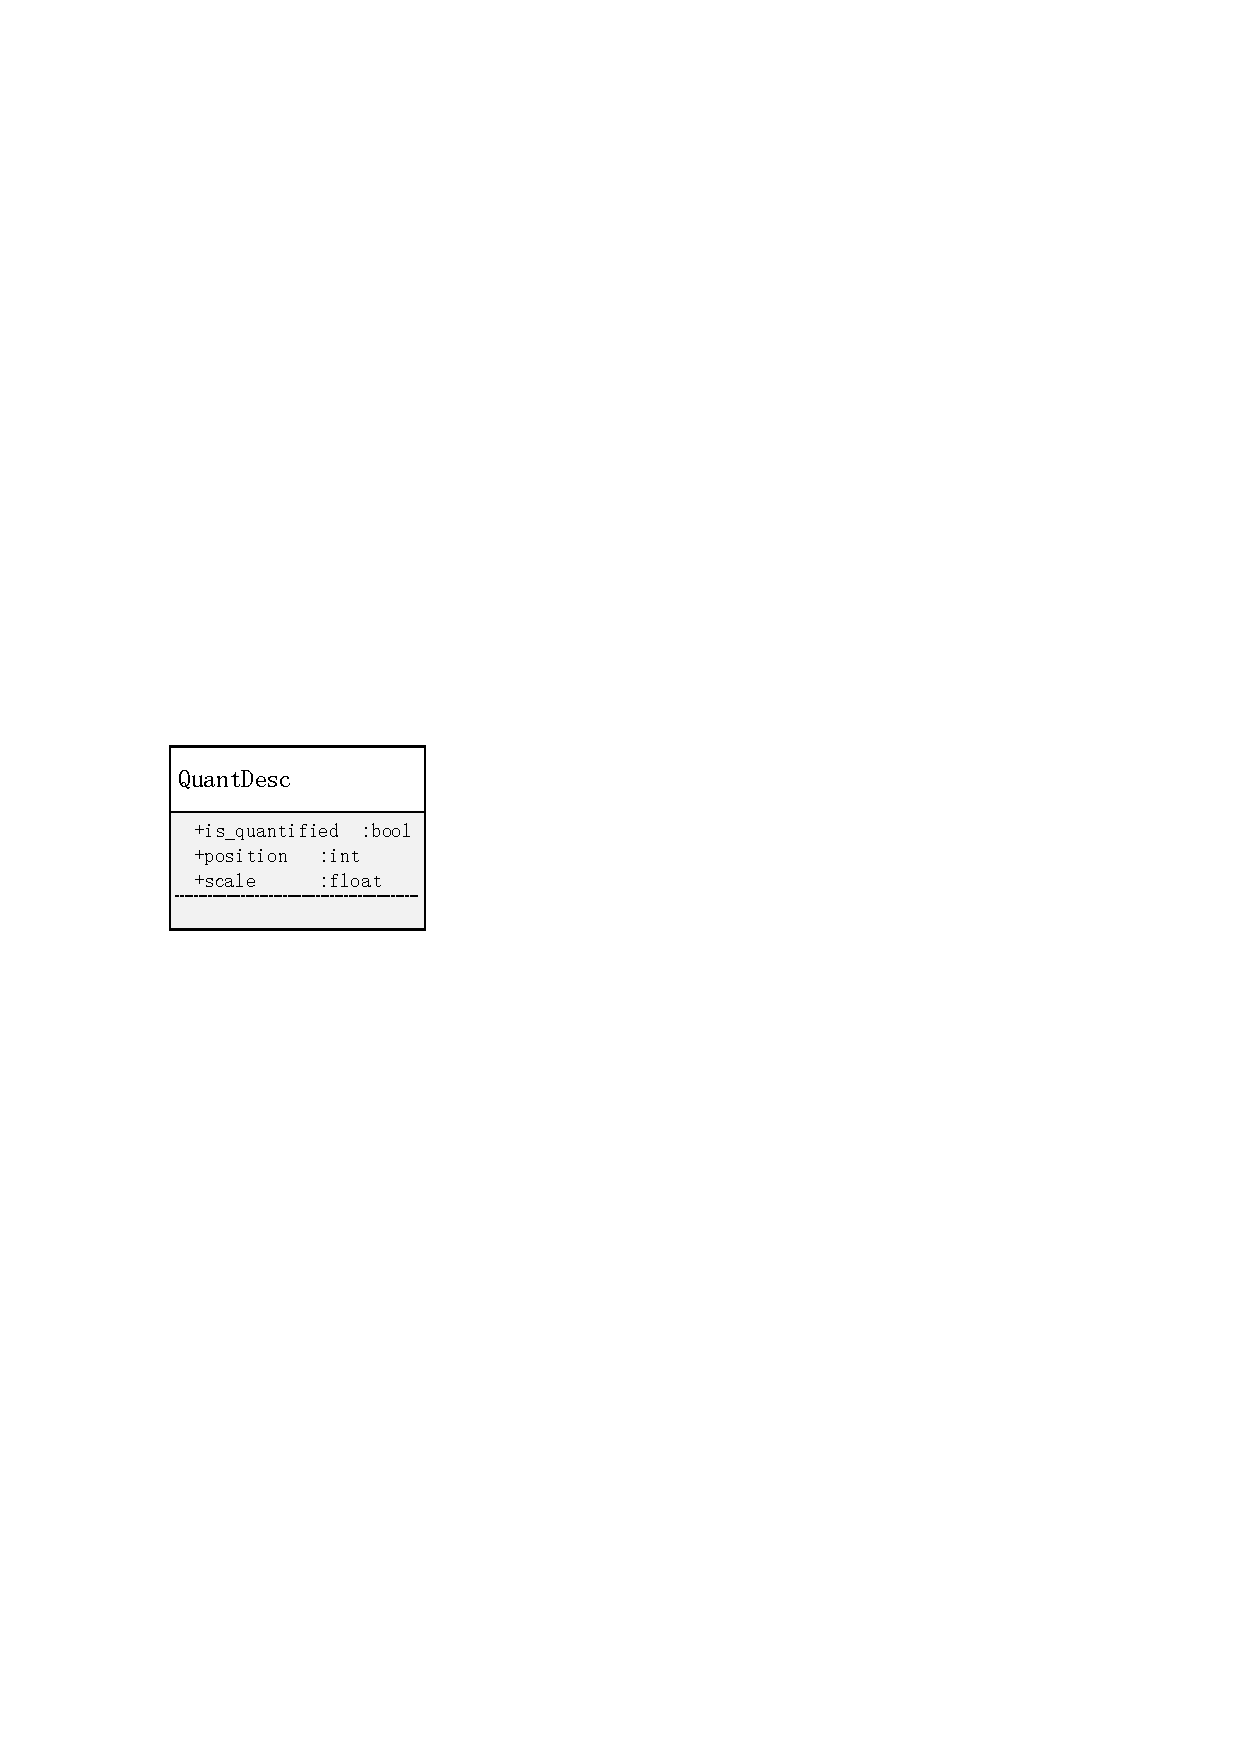
\includegraphics[width=0.4\textwidth]{quant_desc.pdf}
  \caption{量化信息图}
  \label{fig:quant-desc}
\end{figure}

QuantDesc中is\_quantified用来判断数据是否被量化,默认值是false,position和scale用来保存量化参数,默认值分别是0和1.0。
权值量化的过程如图~\ref{fig:weight-quant-process}所示。

\begin{figure}[htb]
  \centering
  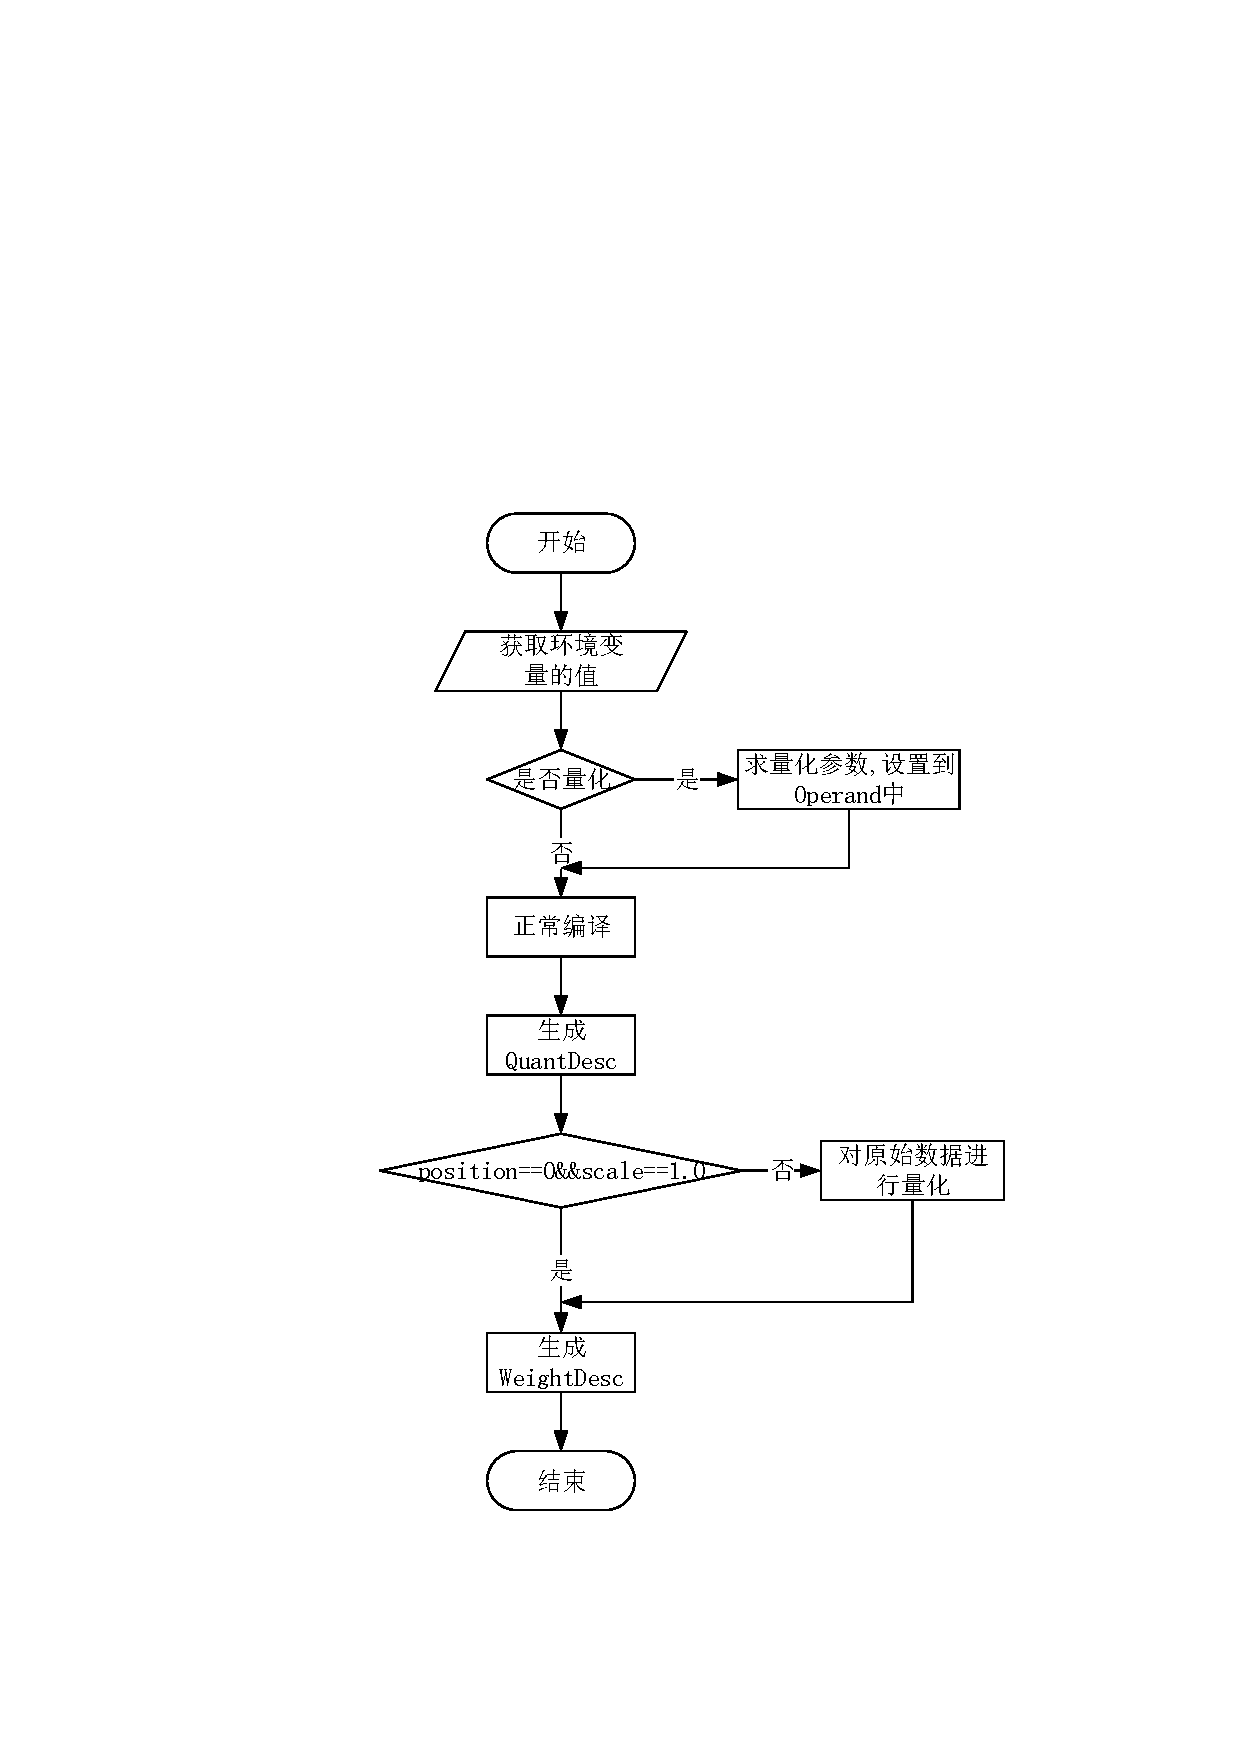
\includegraphics[width=0.4\textwidth]{weight_quant_process.pdf}
  \caption{权值量化流程图}
  \label{fig:weight-quant-process}
\end{figure}

在整个编译生成Kernel的过程中,在两处进行了是否量化的判断,一开始是在编译一开始获取用户计算图的过程中,根据环境变量的值进行判断,如果用户开启了权值量化功能,则求出量化参数并保存到对应的张量中。之后在编译后期生成Kernel的WeightDesc的时候,如果采用了权值量化,则需要对原始数据进行量化处理,将量化后的结果保存到WeightDesc的数据域中。

\section {本章小结}

本章以类图为主,详细介绍了各个模块的实现方式,类之间的关系和接口调用,对于某些比较的复杂的接口,利用流程详细描述其实现逻辑和细节。为了将重点放在模块功能的实现上,在某些模块的设计中,忽略某些不必要的细节,从而突出整体的流程和实现。